\documentclass[12pt,a5paper,twoside]{book}  % use oneside to avoid blank pages

\usepackage[a5paper, top=1.5cm, bottom=2cm, inner=2cm, outer=1.2cm]{geometry}

\usepackage{xcolor}
\usepackage{pagecolor}
\usepackage{graphicx}
\usepackage{fontspec}
\usepackage{polyglossia}
\setmainlanguage{punjabi}
\usepackage{enumitem}
\usepackage{ragged2e}
\usepackage{subcaption}
\usepackage[utf8]{inputenc}
\usepackage{xcolor} % For color support
\usepackage{tikz}   % For drawing the border
\usepackage{eso-pic} % To repeat the drawing on every page
\setlist{topsep=0.3em, itemsep=0.3em}

\newfontfamily\punjabifont[Script=Gurmukhi,
  BoldFont=NotoSerifGurmukhi-SemiBold.ttf
]{NotoSerifGurmukhi-Regular.ttf}

\usepackage{fancyhdr}
\pagestyle{fancy}
\fancyhf{}
\fancyfoot[C]{\thepage}
\renewcommand{\headrulewidth}{0pt}
\renewcommand{\footrulewidth}{0pt}
\definecolor{nanak_niwas_midnight_violet}{HTML}{241236}
\definecolor{nanak_niwas_thistle}{HTML}{D8CCE6}
\definecolor{nanak_niwas_soft_peach}{HTML}{F2D6A2}
\definecolor{nanak_niwas_metalic_gold}{HTML}{D4AF37}
\newcommand{\currentBorderColor}{nanak_niwas_metalic_gold}

\usepackage{setspace}
\setstretch{1.25}  % reduce slightly from 1.4 to avoid overflow

\usepackage{titlesec}
\titleformat{\chapter}[block]
  {\centering\Huge\bfseries\punjabifont}
  {}
  {0pt}
  {}
\titlespacing*{\chapter}{0pt}{0pt}{1em}

% Remove forced page break before chapters
\usepackage{etoolbox}
\makeatletter
\patchcmd{\chapter}
  {\if@openright\cleardoublepage\else\clearpage\fi}
  {\clearpage}{}{}
\makeatother

\AddToShipoutPictureBG{%
  \begin{tikzpicture}[remember picture, overlay]
    \draw[line width=3pt, color=\currentBorderColor] 
      ([shift={(0.7cm, 0.7cm)}]current page.south west) 
      rectangle 
      ([shift={(-0.7cm, -0.7cm)}]current page.north east);
  \end{tikzpicture}%
}


\begin{document}

{\punjabifont

\begin{titlepage}
    \newpagecolor{nanak_niwas_midnight_violet}
    \color{nanak_niwas_metalic_gold}
    \thispagestyle{empty}
    
    % Adjust margins for the cover specifically
    \newgeometry{top=2cm, bottom=2cm, left=1.5cm, right=1.5cm}
    \centering
    
    {\large \bfseries ੴ ਸਤਿਗੁਰ ਪ੍ਰਸਾਦ \par}
    
    % Top padding
    \vspace*{1cm}

    % Image with a subtle frame effect
    \fboxsep=0pt
    \fboxrule=0.5pt
    \fbox{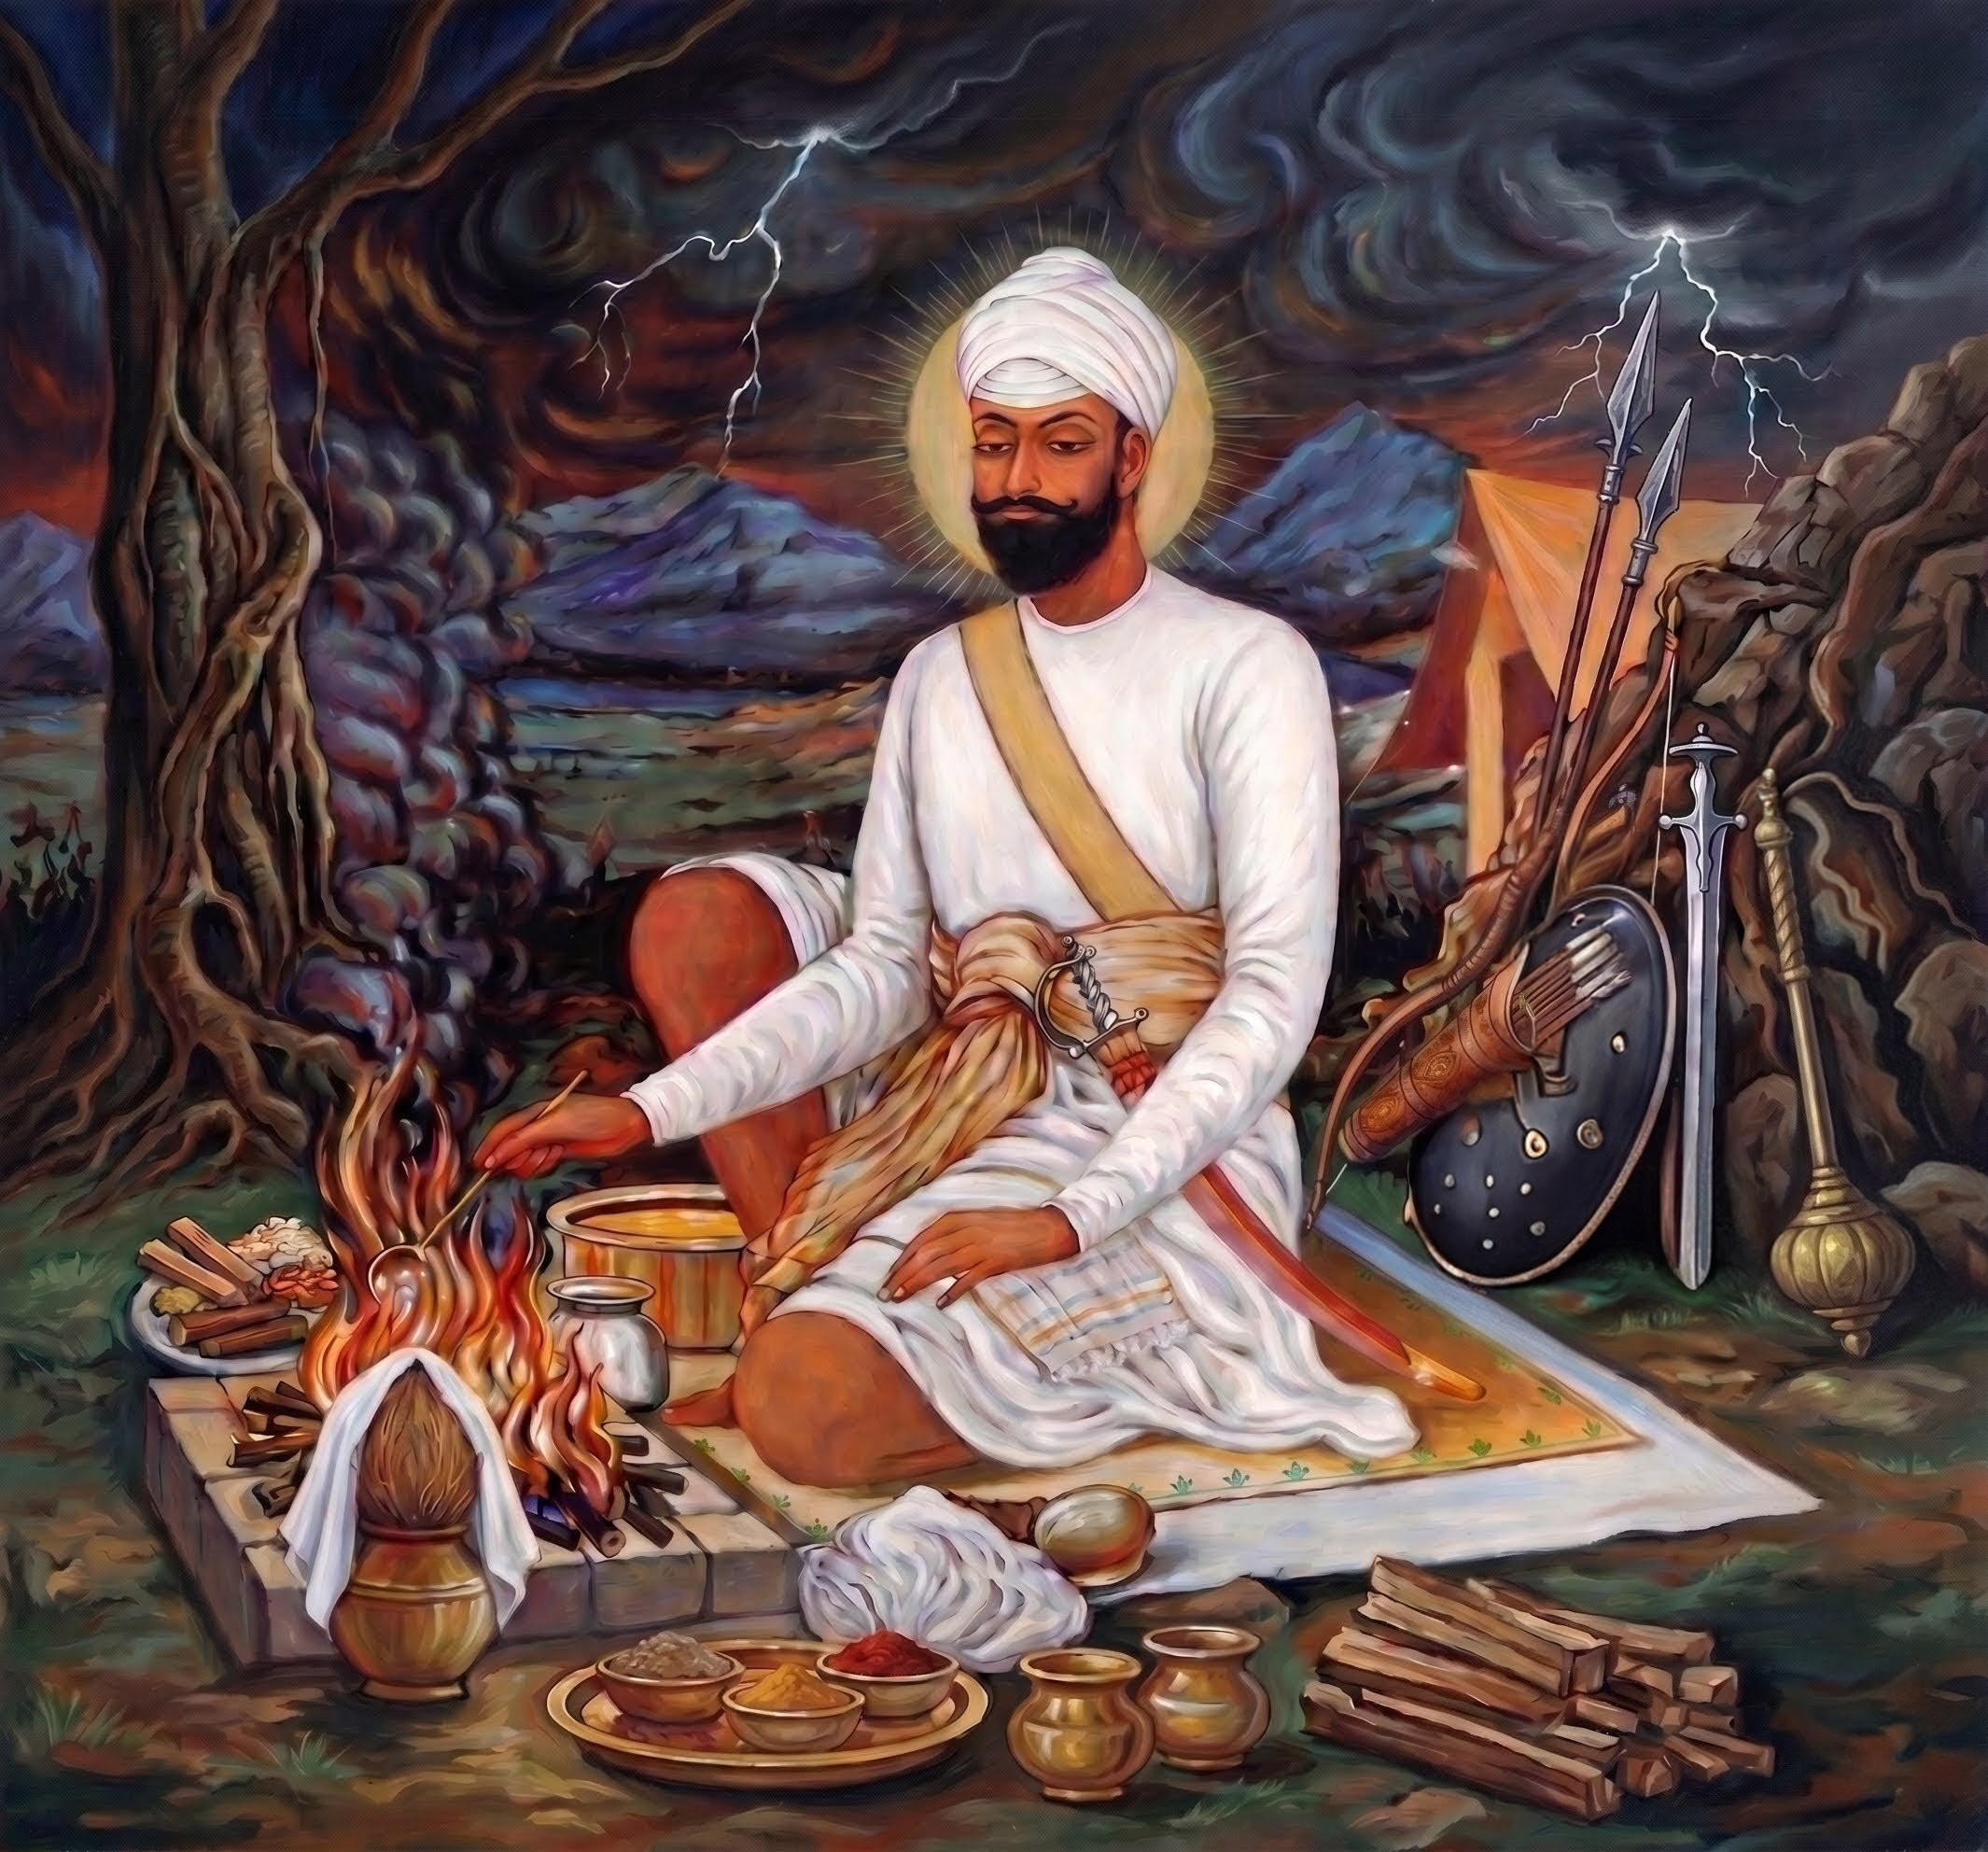
\includegraphics[width=0.85\textwidth]{cover.jpg}}

    \vfill % Pushes content apart naturally

    % Title Section
    {\Huge \bfseries ਹਵਨ \\
    ਇੱਕ ਪੁਰਾਤਨ ਮਰਰਯਾਦਾ \par}
    \vfill
    \fbox{
\includegraphics[width=0.2\textwidth]{nanak_nivas.png}}
    \restoregeometry
\end{titlepage}
\restorepagecolor 
\renewcommand{\currentBorderColor}{nanak_niwas_midnight_violet}  % Ensures TOC starts on a fresh right-hand page (book style)
\null             % Produces a blank page
\thispagestyle{empty}  % Removes page number
\newpage
\tableofcontents
\chapter*{ਭੂਮਿਕਾ}
\addcontentsline{toc}{chapter}{ਭੂਮਿਕਾ}
ਮੈਂ ਮਾਤਾ ਸਾਹਿਬ ਦੇਵਾਂ ਜੀ ਦੇ ਚਰਨ ਕਮਲਾਂ ਵਿਚ ਨਿਮਰਤਾ ਸਹਿਤ ਪ੍ਰਣਾਮ ਕਰਦਾ ਹਾਂ ਅਤੇ ਇਸ ਪੁਸਤਕ ਨੂੰ ਸੇਵਾ ਵਜੋਂ ਭੇਟ ਕਰਦਾ ਹਾਂ। ਬ੍ਰਹਮ ਸ਼ਕਤੀ ਦੇ ਬਗੈਰ ਮੈਂ ਹਿੱਲਣ ਦੇ ਵੀ ਯੋਗ ਨਹੀਂ ਸੀ। ਇਹ ਉਹ ਸ਼ਕਤੀ ਹੈ ਜਿਹਨਾਂ ਦੇ ਸਹਿਯੋਗ ਦੇ ਨਾਲ ਇਹ ਕਿਤਾਬ ਲਿਖੀ ਗਈ ਹੈ। ਮੈਂ ਫੇਰ ਆਪਣਾ ਸੀਸ ਧੰਨ ਗੁਰੂ ਨਾਨਕ ਦੇਵ ਸਾਹਿਬ ਜੀ ਨਿਰੰਕਾਰ ਨੂੰ ਭੇਟ ਕਰਦਾ ਹਾਂ ਜੋ ਮੇਰੇ ਮਾਰਗ ਦਰਸ਼ਕ ਹਨ। ਫੇਰ ਮੈਂ ਆਪਣੀ ਫ਼ਤਿਹ ਧੰਨ ਬਾਬਾ ਸ੍ਰੀ ਚੰਦ ਸਾਹਿਬ ਜੀ (ਧੰਨ ਗੁਰੂ ਨਾਨਕ ਦੇਵ ਸਾਹਿਬ ਜੀ ਦੇ ਸਾਹਿਬਜ਼ਾਦੇ) ਨੂੰ ਭੇਟ ਕਰਦਾ ਹਾਂ ਜਿਹਨਾਂ ਨੇ ਮੇਰੇ ਅੰਦਰ ਪੁਰਾਤਨ ਮਰਯਾਦਾ ਨੂੰ ਜਿਉਂਦਾ ਰੱਖਿਆ।
\\
ਧੰਨ ਬਾਬਾ ਸਰੀ ਚੰਦ ਜੀ ਮਹਾਰਾਜ, ਧੰਨ ਬਾਬਾ ਬਲਵੰਤ ਪਸੰਘ ਜੀ (ਪਸਹੜਾ ਸਾਪਹਬ), ਧੰਨ
ਬਾਬਾ ਪਵਰਸਾ ਪਸੰਘ ਜੀ (ਗੋਪਬੰਦ ਸਦਨ) ਪਜਨਹਾ ਦੇ ਦਾਸ ਦੇ ਪਸਰ ਤੇ ਹੱਥ ਰਖ ਕੇ ਇਹ
ਗਰੰਥ ਦੀ ਸੇਵਾ ਕਰਾਈ ਹੈ । 
\\
ਮੈਂ ਸਾਧ ਸੰਗਤ (ਸਰਦਾਰ ਚਰਨਪ੍ਰੀਤ ਸਿੰਘ, ਬੀਬੀ ਗੁਰਿੰਦਰ ਕੌਰ, ਬੀਬੀ ਹਰਸ਼ੀਨ ਕੌਰ, ਬੀਬੀ ਜਸਲੀਨ ਕੌਰ) ਅਤੇ ਆਪਣੇ ਮਾਤਾ ਪਿਤਾ ਜੀ ਦਾ ਧੰਨਵਾਦ ਕਰਦਾ ਹਾਂ ਜਿਹਨਾਂ ਦੇ ਸਹਿਯੋਗ ਨਾਲ ਇਸ ਪੁਸਤਕ ਵਿਚ ਮੌਜੂਦ ਜਾਣਕਾਰੀ ਇਕੱਠੀ ਕੀਤੀ ਗਈ। ਜੇ ਸੰਗਤਾਂ ਨੂੰ ਇਸ ਕੰਮ ਵਿੱਚ ਕੋਈ ਕਮੀਆਂ ਨਜ਼ਰ ਆਉਂਦੀਆਂ ਹਨ ਤਾਂ ਉਹ ਸਿਰਫ਼ ਮੇਰੀਆਂ ਹਨ, ਕਿਰਪਾ ਕਰਕੇ ਮੈਨੂੰ ਮੁਆਫ਼ ਕਰਨਾ ਅਤੇ ਦਾਸ ਨੂੰ ਆਪਣੇ ਵਿਚਾਰ ਜ਼ਰੂਰ ਭੇਜਣਾ।
\newpage
ਇਹ ਸੇਵਾ ਨਾਨਕ ਨਿਵਾਸ ਵੱਲੋਂ ਨਿਮਾਣੇ ਰੂਪ ਵਿੱਚ ਭੇਟ ਕੀਤੀ ਗਈ ਹੈ। ਇਸ ਵਿਸ਼ੇਸ਼ ਦਸਤਾਵੇਜ਼ ਦੀ ਸੇਵਾ ਹੇਠ ਲਿਖੇ ਸੇਵਾਦਾਰਾਂ ਵੱਲੋਂ ਪੂਰੀ ਸ਼ਰਧਾ ਨਾਲ ਕੀਤੀ ਗਈ ਹੈ:
\begin{itemize}
    \item ਭਾਈ ਮਨਪ੍ਰੀਤ ਸਿੰਘ
    \item ਭਾਈ ਅਕਾਲੀ ਸੁਰਜੀਤ ਸਿੰਘ
    \item ਅਨਮੋਲ ਦੀਪ ਸਿੰਘ
    \item ਜਯ ਸਿੰਘ (ਭਟਕਦੀ ਆਤਮਾ)
\end{itemize}
\begin{center}
।।ਦੋਹਰਾ।।
\\
ਆਦਿ ਗੁਰੂ ਤੇ ਦਸਮ ਲੋਹ ਗ੍ਰੰਥ ਪੰਥ ਕੀ ਟੇਕ ਗਾਹੇ
\\
ਪੂਰਨ ਥਿਯਾ ਗ੍ਰੰਥ ਯਹ ਦਯਾ ਸਰਬ ਹਰ ਇਕ 
\\
\end{center}
\begin{FlushRight}
\textbf{-ਗਿਆਨੀ ਗਿਆਨ ਸਿੰਘ}
\\
\textbf{ਨਵੀਨ ਪੰਥ ਪ੍ਰਕਾਸ਼}
\end{FlushRight}
\clearpage
\chapter*{ਨਾਨਕ ਨਿਵਾਸ}
\addcontentsline{toc}{chapter}{ਨਾਨਕ ਨਿਵਾਸ}
ਨਾਨਕ ਨਿਵਾਸ ਇੱਕ ਗੁਰਮਤਿ ਵਿਦਿਆਲਿਆ ਹੈ ਜਿਸਦਾ ਮਕਸਦ ਗੁਰੂ ਨਾਨਕ ਦੇਵ ਜੀ ਦੀ ਅਦਵੈਤ ਅਤੇ ਪ੍ਰੇਮ ਦੀ ਸਿੱਖਿਆ ਨੂੰ ਸਾਂਝਾ ਕਰਨਾ ਹੈ, ਅਤੇ ਖੋਜੀਆਂ ਨੂੰ ਆਪਣੇ ਅਸਲ ਸਰੂਪ ਨੂੰ ਸਮਝਣ ਵਿੱਚ ਮਦਦ ਕਰਨਾ ਹੈ।
\\
ਬ੍ਰਹਮ ਵਿਦਿਆ ਦੀਆਂ ਕਲਾਸਾਂ ਹਰ ਹਫਤੇ ਆਨਲਾਈਨ ਪੰਜਾਬੀ, ਹਿੰਦੀ ਅਤੇ ਅੰਗ੍ਰੇਜ਼ੀ ਵਿੱਚ ਹੁੰਦੀਆਂ ਹਨ, ਜਿਥੇ ਅਸੀਂ ਪੁਰਾਤਨ ਗ੍ਰੰਥਾਂ ਨੂੰ ਗੁਰਮਤਿ ਦੀ ਨਜ਼ਰ ਨਾਲ ਸਮਝਦੇ ਹਾਂ ਅਤੇ ਇਹ ਵੇਖਦੇ ਹਾਂ ਕਿ ਇਹ ਗਿਆਨ ਅਸੀਂ ਆਪਣੀ ਰੋਜ਼ਾਨਾ ਜ਼ਿੰਦਗੀ ਵਿੱਚ ਕਿਵੇਂ ਲਾਗੂ ਕਰ ਸਕਦੇ ਹਾਂ। ਇਸਦੇ ਨਾਲ ਨਾਲ, ਅਸੀਂ ਕਾਵਿ ਵਿਦਿਆ ਦੀਆਂ ਆਨਲਾਈਨ ਕਲਾਸਾਂ ਵੀ ਕਰਵਾਉਂਦੇ ਹਾਂ ਅਤੇ ਮੇਲਬਰਨ ਵਿੱਚ ਹਰ ਮਹੀਨੇ ਸੰਗਤ ਦੇ ਸੈਸ਼ਨ ਰੱਖਦੇ ਹਾਂ, ਜਿਥੇ ਸਿੱਖਣ, ਜੁੜਨ ਅਤੇ ਇਕੱਠੇ ਵਧਣ ਦਾ ਮੌਕਾ ਮਿਲਦਾ ਹੈ।
\\
ਨਾਨਕ ਨਿਵਾਸ ਹਰ ਉਸ ਵਿਅਕਤੀ ਲਈ ਹੈ ਜੋ ਸੱਚ ਦੀ ਖੋਜ ਵਿੱਚ ਹੈ, ਕਿਸੇ ਇੱਕ ਸਮਾਜ ਜਾਂ ਸੰਪ੍ਰਦਾ ਤੱਕ ਸੀਮਤ ਨਹੀਂ। ਸਾਲ ਭਰ ਅਸੀਂ ਵੱਖ-ਵੱਖ ਸਮਾਗਮ ਵੀ ਕਰਦੇ ਹਾਂ ਤਾਂ ਕੀ ਸੰਗਤ ਨਾਲ ਹੋਰ ਜੁੜ ਸਕੀਏ ਅਤੇ ਇਹ ਸੰਦੇਸ਼ ਸਾਂਝਾ ਕਰ ਸਕੀਏ, ਨਾਲ ਹੀ ਸੰਗਤਾਂ ਨੂੰ ਆਪਣੀ ਖੁਦ ਦੀ ਖੋਜ ਕਰਨ ਲਈ ਪ੍ਰੇਰਿਤ ਕਰਦੇ ਹਾਂ ਤਾਂ ਕੀ ਉਹ ਸਿਰਫ਼ ਮੰਨਣ ਦੀ ਬਜਾਏ ਇਸਨੂੰ ਆਪਣੀ ਜ਼ਿੰਦਗੀ ਵਿੱਚ ਜੀ ਸਕਣ।
\begin{figure}[h]
      \centering
      
\includegraphics[width=4cm,keepaspectratio]{nanak_nivas.png}
    \end{figure}
\clearpage
\chapter*{ਹਵਨ ਕੀ ਹੈ?}
\addcontentsline{toc}{chapter}{ਹਵਨ ਕੀ ਹੈ?}
ਇਹ ਪੁ ਤਕ ਖਾਲ ਾ ਪਿੰਥ ਦੀ ਪੁਰਾਤਨ ਹਵਨ ਪਰਿੰਪਰਾ ਨੂੰ ੁਰਜੀਤ ਕਰਨ ਅਤੇਉ ਰਵਚ ਰੌਸ਼ਨੀ
ਰਲਆਉਣ ਦਾ ਇੱਕ ਉਪਰਾਲਾ ਹ , ਜ ਰਕ ਦਲ ਪਿੰਥ (ਬੁੱਢਾ ਦਲ ਅਤੇਤਰਨਾ ਦਲ) ਅਤੇਹ ਰ ਰਨਹਿੰਗ
ਰ ਿੰਘ ਿੰਪਰਦਾਵਾਂ ਰਵਚ ਅਜੇਵੀ ਚਲਾਈ ਜਾਂਦੀ ਹ । ਾਲਾਂ ਦੌਰਾਨ, ਖਾਲ ੇਰਵੱਚ ਨ ੧੮੭੦ ਰਵਚ
ਸ਼ੁਰੂਹ ਈ ਰ ਿੰਘ ਭਾ ਲਰਹਰ ਦੇਨੁਕ ਾਨ ਰਵੱਚ ਇੱਕ ੀ। ਰਕਉੈਂਰਕ ਕੁਝ ਅਰਭਆ ਜ ਪੁਰਾਤਨ
ਰ ੱਖਾਂ ਦੁਆਰਾ ਕੀਤੇਜਾਂਦੇ ੀ ਉਹਨਾਂ ਨੂੰ ਰਨਰਉਤਸ਼ਾਰਹਤ ਕੀਤਾ ਅਤੇਰਹਿੰਦੂਆਂ ਦੀ ਪਰਿੰਪਰਾ ਅਤੇ
ਕੁਝ ਮੁ ਲਮਾਨਾਂ ਦੀ ਪਰਿੰਪਰਾ ਕਰਹ ਕੇਬਰਖਾ ਤ ਕੀਤਾ ਰਗਆ। ਇਹ ਪੁ ਤਕ ਇ ਗੱਲ ਦੀ
ਡੂਿੰਘਾਈ ਨਾਲ ਖ ਜ ਨਹੀੈਂ ਕਰੇਗੀ ਰਕ ਰ ਿੰਘ ਭਾ ਲਰਹਰ ਦੇਕਾਰਨ ਕੀ ਅਤੇਰਕਵੇੈਂ ਵਾਪਰਰਆ, ਪਰ
ਹਵਨ ਦੀ ਪਰਿੰਪਰਾ ਅਤੇਗੁਰਮਰਤ ਅਤੇਰਵਰਗਆਰਨਕ ਪੱਖ ੈਂ ਇ ਦੀ ਮਹੱਤਤਾ ਤੇਜ ਰ ਰਦੱਤਾ
ਜਾਵੇਗਾ। ਰਜਵੇੈਂ ਰਕ ਹਵਨ ਨੂੰ ਰਹਿੰਦੂਆਂ ਵੱਲ ੈਂ ਵੱਡੇਪੱਧਰ ਤੇਅਰਭਆ ਕਰਨ ਲਈ ਜਾਰਣਆ ਜਾਂਦਾ
ਹ , ਉਹਨਾਂ ਦੀ ਪਰਿੰਪਰਾ ਦਾ ਕੁਝ ਹਵਾਲਾ ਵੀ ਤੁਲਨਾ ਦੇਅਧਾਰ ਤੇਰ ੱਟਾ ਕੱਢਣ ਲਈ ਬਣਾਇਆ
ਜਾਵੇਗਾ।
\\

\chapter*{ਬਿਬੇਕ ਮਰਯਾਦਾ}
\addcontentsline{toc}{chapter}{ਬਿਬੇਕ ਮਰਯਾਦਾ}
ਬਿਬੇਕ ਮਰਯਾਦਾ ਦੇ ਮੁੱਖ ਨਿਯਮ ਹੇਠ ਲਿਖੇ ਅਨੁਸਾਰ ਹਨ:
\begin{itemize}
    \item \textbf{ਲੰਗਰ ਦੀ ਮਰਯਾਦਾ:} ਗੁਰੂ ਕੇ ਲੰਗਰ ਤੋਂ ਹਮੇਸ਼ਾ ਤਾਜ਼ਾ ਅਤੇ ਹਲਕਾ ਭੋਜਨ ਹੀ ਛਕਣਾ ਚਾਹੀਦਾ ਹੈ।
    \item \textbf{ਰਸਨਾ ਦੀ ਸੰਜਮ: }ਸੰਗਤ ਵਿੱਚ ਰਹਿੰਦਿਆਂ ਬੇਲੋੜੀ ਗੱਲਬਾਤ ਕਰਨ ਤੋਂ ਪਰਹੇਜ਼ ਕਰੋ। ਕੇਵਲ ਸੇਵਾ ਦੇ ਕਾਰਜ ਲਈ ਜਿੰਨੀ ਲੋੜ ਹੋਵੇ, ਉਨੀ ਹੀ ਗੱਲ ਕਰਨੀ।
    \item \textbf{ਸਰਬਲੋਹ ਦੀ ਵਰਤੋਂ:} ਭੋਜਨ ਤਿਆਰ ਕਰਨ (ਬਿਬੇਕੀ ਦੇਗ) ਅਤੇ ਛਕਣ ਲਈ ਕੇਵਲ ਸਰਬਲੋਹ (ਲੋਹੇ) ਦੇ ਬਰਤਨਾਂ ਦੀ ਹੀ ਵਰਤੋਂ ਕਰਨੀ।
    \item \textbf{ਬਰਤਨਾਂ ਦੀ ਸਫਾਈ:} ਸਰਬਲੋਹ ਦੇ ਬਰਤਨਾਂ ਨੂੰ ਮਾਂਜਣ ਅਤੇ ਸਾਫ਼ ਕਰਨ ਲਈ ਕੇਵਲ ਸੁਆਹ ਜਾਂ ਰੇਤ ਦੀ ਵਰਤੋਂ ਕਰਨੀ।
    \item \textbf{ਸਣੇ ਕੇਸੀ ਇਸ਼ਨਾਨ:} ਹਰ ਰੋਜ਼ ਕੇਸਾਂ ਸਮੇਤ (ਸਣੇ ਕੇਸੀ) ਇਸ਼ਨਾਨ ਕਰਨਾ ਲਾਜ਼ਮੀ ਹੈ।
    \item \textbf{ਲਘੂ ਸ਼ੰਕਾ ਤੋਂ ਬਾਅਦ ਸੋਧ:} ਪਿਸ਼ਾਬ (ਲਘੂ ਸ਼ੰਕਾ) ਕਰਨ ਤੋਂ ਬਾਅਦ ਗੋਡਿਆਂ ਅਤੇ ਬਾਹਾਂ ਤੱਕ ਜਲ ਨਾਲ ਚੰਗੀ ਤਰ੍ਹਾਂ ਸੋਧ (ਸਫਾਈ) ਕਰਨੀ।
    \item \textbf{ਪੂਰਨ ਇਸ਼ਨਾਨ:} ਜੰਗਲ ਪਾਣੀ (ਸ਼ੌਚ) ਜਾਣ ਤੋਂ ਬਾਅਦ ਸਰੀਰ ਦਾ ਪੂਰਨ ਇਸ਼ਨਾਨ ਕਰਨਾ ਜ਼ਰੂਰੀ ਹੈ।
\end{itemize}
\chapter*{ਸੇਵਾਵਾਂ ਅਤੇ ਸੇਵਾਦਾਰਾਂ ਦਾ ਵੇਰਵਾ}
\addcontentsline{toc}{chapter}{ਸੇਵਾਵਾਂ ਅਤੇ ਸੇਵਾਦਾਰਾਂ ਦਾ ਵੇਰਵਾ}
ਅਖੰਡ ਪਾਠ ਨੂੰ ਨਿਰਵਿਘਨ ਅਤੇ ਮਰਯਾਦਾ ਅਨੁਸਾਰ ਸੰਪੂਰਨ ਕਰਨ ਲਈ ਹੇਠ ਲਿਖੀਆਂ ਸੇਵਾਵਾਂ ਅਤੇ ਸੇਵਾਦਾਰਾਂ ਦੀ ਉਚਿਤ ਗਿਣਤੀ ਬਹੁਤ ਜ਼ਰੂਰੀ ਹੈ। 
\begin{center}
    \textbf{ਸਾਰੇ ਸੇਵਾਦਾਰਾਂ ਦਾ ਬਿਬੇਬਕੀ ਮਰਯਾਦਾ ਵਿਚ ਹੋਣਾ ਜ਼ਰੂਰੀ ਹੈ}
\end{center}
\begin{itemize}
    \item \textbf{ਪਾਠੀ ਸਿੰਘਾਂ ਦੀ ਸੇਵਾ (ਗਿਣਤੀ: 5 - 10 ਜਾਂ ਵੱਧ)} ਪਾਠੀ ਸਿੰਘਾਂ ਦੀ ਗਿਣਤੀ ਇਸ ਲਈ ਜ਼ਿਆਦਾ ਰੱਖੀ ਜਾਂਦੀ ਹੈ ਤਾਂ ਜੋ ਹਰ ਪਾਠੀ ਸਿੰਘ ਆਪਣੀ ਵਾਰੀ (ਰੌਲ) ਅਨੁਸਾਰ ਆਰਾਮ ਕਰ ਸਕੇ ਅਤੇ ਪਾਠ ਦੌਰਾਨ ਇਕਾਗਰਤਾ ਅਤੇ ਸ਼ੁੱਧ ਉਚਾਰਨ ਬਣਿਆ ਰਹੇ। ਆਮ ਤੌਰ 'ਤੇ ਇੱਕ ਰੌਲ ਦੋ ਘੰਟੇ ਦੀ ਹੁੰਦੀ ਹੈ।
    \item \textbf{ਚੌਰ ਸਾਹਿਬ ਦੀ ਸੇਵਾ (ਗਿਣਤੀ: 1)} ਜਿੰਨਾ ਚਿਰ ਪਾਠ ਚੱਲਦਾ ਹੈ, ਉਨਾ ਚਿਰ ਗ੍ਰੰਥ ਦੇ ਤਾਬਿਆ ਵਿੱਚ ਬੈਠ ਕੇ ਚੌਰ ਸਾਹਿਬ ਦੀ ਸੇਵਾ ਨਿਰੰਤਰ ਹੋਣੀ ਚਾਹੀਦੀ ਹੈ। ਇਹ ਸੇਵਾ ਗ੍ਰੰਥ ਦੇ ਪ੍ਰਤੀ ਅਦਬ ਅਤੇ ਸਤਿਕਾਰ ਦਾ ਪ੍ਰਤੀਕ ਹੈ। ਪਾਠੀ ਸਿੰਘ ਦੇ ਨਾਲ ਇੱਕ ਵੱਖਰਾ ਸੇਵਾਦਾਰ ਇਸ ਸੇਵਾ ਲਈ ਹਮੇਸ਼ਾ ਹਾਜ਼ਰ ਰਹਿਣਾ ਚਾਹੀਦਾ ਹੈ।
    \item \textbf{ਧੂਪ ਅਤੇ ਸੁਗੰਧ ਸੇਵਾ (ਗਿਣਤੀ: 1)} ਇਸ ਸੇਵਾਦਾਰ ਦੀ ਜ਼ਿੰਮੇਵਾਰੀ ਹੁੰਦੀ ਹੈ ਕਿ ਉਹ ਕੋਲਿਆਂ ਨੂੰ ਭਖਦਾ ਰੱਖੇ ਅਤੇ ਸਮੇਂ-ਸਮੇਂ ਸਿਰ ਗੁੱਗਲ, ਚੰਦਨ ਅਤੇ ਘਿਓ ਦੀ ਵਰਤੋਂ ਕਰਕੇ ਵਾਤਾਵਰਣ ਨੂੰ ਸੁਗੰਧਿਤ ਬਣਾਈ ਰੱਖੇ। ਇਸ ਨਾਲ ਪਾਠ ਵਾਲੇ ਅਸਥਾਨ 'ਤੇ ਇਕਾਗਰਤਾ ਬਣੀ ਰਹਿੰਦੀ ਹੈ ਅਤੇ ਮਨ ਨੂੰ ਸ਼ਾਂਤੀ ਮਿਲਦੀ ਹੈ।
    \item \textbf{ਪਹਿਰੇਦਾਰੀ ਦੀ ਸੇਵਾ (ਗਿਣਤੀ: 1 - 2)} ਪਹਿਰੇਦਾਰ ਦੀ ਮੁੱਖ ਜ਼ਿੰਮੇਵਾਰੀ ਅਖੰਡ ਪਾਠ ਦੀ ਮਰਯਾਦਾ ਅਤੇ ਸ਼ਾਂਤੀ ਕਾਇਮ ਰੱਖਣਾ ਹੈ। ਉਹ ਯਕੀਨੀ ਬਣਾਉਂਦਾ ਹੈ ਕਿ ਸੇਵਾਦਾਰ ਬਿਬੇਕ ਨਿਯਮਾਂ ਦੀ ਸਖ਼ਤੀ ਨਾਲ ਪਾਲਣਾ ਕਰਨ, ਜਿਵੇਂ ਕਿ ਲੰਗਰ ਤੋਂ ਤਾਜ਼ਾ ਭੋਜਨ ਛਕਣਾ, ਸਰਬਲੋਹ ਦੇ ਬਰਤਨਾਂ ਨੂੰ ਸੁਆਹ ਨਾਲ ਮਾਂਜਣਾ, ਸਣੇ ਕੇਸੀ ਇਸ਼ਨਾਨ ਕਰਨਾ ਅਤੇ ਪਖਾਨੇ ਤੋਂ ਬਾਅਦ ਪੂਰਨ ਸੁੱਚਮਤਾ (ਇਸ਼ਨਾਨ ਤੇ ਸੋਧ) ਰੱਖਣੀ। ਬੇਲੋੜੀ ਗੱਲਬਾਤ ਰੋਕ ਕੇ ਅਤੇ ਅਨੁਸ਼ਾਸਨ ਬਣਾ ਕੇ ਉਹ ਪਾਠ ਦੀ ਪਵਿੱਤਰਤਾ ਵਿੱਚ ਕੋਈ ਵਿਘਨ ਨਹੀਂ ਪੈਣ ਦਿੰਦਾ।
    \item \textbf{ਲੰਗਰ ਅਤੇ ਜਲ-ਪਾਣੀ ਦੀ ਸੇਵਾ (ਗਿਣਤੀ: 3 - 5)} ਇਹ ਟੀਮ ਪਾਠੀ ਸਿੰਘਾਂ ਅਤੇ ਆਈ ਹੋਈ ਸੰਗਤ ਲਈ ਸਮੇਂ ਸਿਰ ਪ੍ਰਸ਼ਾਦਾ (ਭੋਜਨ), ਚਾਹ ਅਤੇ ਜਲ ਦਾ ਪ੍ਰਬੰਧ ਕਰਦੀ ਹੈ। ਇਨ੍ਹਾਂ ਸੇਵਾਦਾਰਾਂ ਦੀ ਜ਼ਿੰਮੇਵਾਰੀ ਲੰਗਰ ਤਿਆਰ ਕਰਨ ਤੋਂ ਲੈ ਕੇ ਵਰਤਾਉਣ ਅਤੇ ਬਾਅਦ ਵਿੱਚ ਸਫਾਈ ਰੱਖਣ ਤੱਕ ਦੀ ਹੁੰਦੀ ਹੈ।
    \item \textbf{ਮੁੱਖ ਪ੍ਰਬੰਧਕ ਜਾਂ ਸੇਵਾਦਾਰ (ਗਿਣਤੀ: 1)} ਇਹ ਵਿਅਕਤੀ ਪੂਰੇ ਸਮਾਗਮ ਦੀ ਰੀੜ੍ਹ ਦੀ ਹੱਡੀ ਹੁੰਦਾ ਹੈ। ਉਸ ਦੀ ਮੁੱਖ ਜ਼ਿੰਮੇਵਾਰੀ ਇਹ ਦੇਖਣਾ ਹੈ ਕਿ:
    \begin{itemize}
        \item ਸਾਰੇ ਪਾਠੀ ਸਿੰਘ ਸਮੇਂ ਸਿਰ ਆਪਣੀ ਰੌਲ 'ਤੇ ਪਹੁੰਚ ਰਹੇ ਹਨ।
        \item ਸਾਰੀਆਂ ਸੇਵਾਵਾਂ ਸੁਚਾਰੂ ਢੰਗ ਨਾਲ ਚੱਲ ਰਹੀਆਂ ਹਨ।
        \item ਜੇਕਰ ਕਿਸੇ ਚੀਜ਼ ਦੀ ਘਾਟ ਹੋਵੇ, ਤਾਂ ਉਸ ਨੂੰ ਤੁਰੰਤ ਪੂਰਾ ਕਰਨਾ।
    \end{itemize}
\end{itemize}
\chapter*{ਸ੍ਰੀ ਗੁਰੂ ਗ੍ਰੰਥ ਸਾਹਿਬ ਜੀ ਦੇ ਸਹਿਜ ਅਤੇ ਅਖੰਡ ਪਾਠ ਦੀ ਮਰਯਾਦਾ}
\addcontentsline{toc}{chapter}{ਸ੍ਰੀ ਗੁਰੂ ਗ੍ਰੰਥ ਸਾਹਿਬ ਜੀ ਦੇ ਸਹਿਜ ਪਾਠ ਦੀ ਮਰਯਾਦਾ}
\section*{ਆਰੰਭ}
\begin{itemize}
  \item ਅਖੰਡ ਪਾਠ ਅਤੇ ਸਹਿਜ ਪਾਠ ਦੀ ਆਰੰਭਤਾ ਦੀ ਮਰਯਾਦਾ ਇੱਕੋ ਜਿਹੀ ਹੈ
  \item ਸਭ ਤੋਂ ਪਹਿਲਾਂ ਦੇਗ (ਕੜਾਹ ਪ੍ਰਸਾਦ) ਤਿਆਰ ਕਰਕੇ ਰੱਖਣੀ ਹੈ, ਫਿਰ ਅਰਦਾਸ ਕਰਕੇ ਭੋਗ ਲਵਾਉਣਾ ਅਤੇ ਹੁਕਮਨਾਮਾ ਸਾਹਿਬ ਲੈਣਾ ਹੈ
  \item ਇਸ ਤੋਂ ਬਾਅਦ ਪਾਠ ਆਰੰਭ ਕਰਨਾ ਹੈ
  \item ਜਪੁਜੀ ਸਾਹਿਬ (ਪੂਰਾ ਜਾਂ 5 ਪੌੜੀਆਂ) ਦੇ ਜਾਪ ਤੋਂ ਬਾਅਦ ਦੇਗ ਵਰਤਾਉਣੀ ਹੈ
\end{itemize}
\section*{ਮੱਧ}
\begin{itemize}
  \item ਸਹਿਜ ਪਾਠ ਵਿੱਚ ਜਦੋਂ 705 ਅੰਗ 'ਤੇ "ਆਦਿ ਪੂਰਨ ਮਧਿ ਪੂਰਨ ਅੰਤਿ ਪੂਰਨ ਪਰਮੇਸੁਰਹ" ਵਾਲੀ ਪੰਗਤੀ ਆਉਂਦੀ ਹੈ, ਤਾਂ ਉਸ ਪੰਗਤੀ ਤੋਂ ਉੱਪਰਲਾ ਸ਼ਬਦ ਪੜ੍ਹ ਕੇ ਰੁਕ ਜਾਣਾ ਹੈ
  \item ਸਭ ਤੋਂ ਪਹਿਲਾਂ ਦੇਗ (ਕੜਾਹ ਪ੍ਰਸਾਦ) ਤਿਆਰ ਕਰਕੇ ਰੱਖਣੀ ਹੈ, ਫਿਰ ਅਰਦਾਸ ਕਰਕੇ ਭੋਗ ਲਵਾਉਣਾ ਅਤੇ ਹੁਕਮਨਾਮਾ ਸਾਹਿਬ ਲੈਣਾ ਹੈ
  \item ਅਖੰਡ ਪਾਠ ਵਿੱਚ ਵੀ ਇਸੇ ਪੰਗਤੀ 'ਤੇ ਮੱਧ ਦੀ ਅਰਦਾਸ ਕੀਤੀ ਜਾਂਦੀ ਹੈ
  \item ਨੋਟ: ਮੱਧ ਵੇਲੇ ਅਨੰਦ ਸਾਹਿਬ ਦਾ ਪਾਠ ਵੀ ਕਰਨਾ ਚਾਹੀਦਾ ਹੈ ਅਤੇ ਫਿਰ ਅਰਦਾਸ ਤੇ ਹੁਕਮਨਾਮਾ ਲੈਣਾ ਚਾਹੀਦਾ ਹੈ
\end{itemize}
\section*{ਭੋਗ}
\begin{itemize}
    \item ਸਲੋਕ ਮਹਲਾ 5 (ਪੰਨਾ 1426) ਤੋਂ ਬਾਅਦ ਜਦੋਂ "ਪਾਪੀ ਕਰਮ ਕਮਾਵਦੇ ਕਰਦੇ ਹਾਏ ਹਾਏ" ਵਾਲੀ ਪੰਗਤੀ ਆਉਂਦੀ ਹੈ, ਤਾਂ ਉਸ ਤੋਂ ਬਾਅਦ ਗਾ ਕੇ (ਸੁਰ ਵਿੱਚ) ਪੜ੍ਹਨਾ ਹੈ
    \item ਆਰਤੀ ਕਰਨੀ ਹੈ (ਆਦਿ ਮਹਾਰਾਜ ਅਤੇ ਦਸਮ ਮਹਾਰਾਜ ਦੀਆਂ ਬਾਣੀਆਂ ਨਾਲ)
    \item ਇਸ ਤੋਂ ਉਪਰੰਤ ਜਪੁਜੀ ਸਾਹਿਬ ਅਤੇ ਅਨੰਦ ਸਾਹਿਬ ਸੰਪੂਰਨ ਪੜ੍ਹ ਕੇ ਭੋਗ ਦੀ ਅਰਦਾਸ, ਬੇਨਤੀ ਅਤੇ ਹੁਕਮਨਾਮਾ ਸਾਹਿਬ ਲੈਣਾ ਹੈ
    \item ਹੁਕਮਨਾਮਾ ਸਾਹਿਬ ਲਈ ਕੁਝ ਅੰਗ ਅੱਗੇ-ਪਿੱਛੇ ਕਰਕੇ ਜੋ ਵੀ ਸਾਹਮਣੇ ਆਵੇ, ਉਹ ਮੁੱਖ ਵਾਕ ਲੈਣਾ ਹੈ
\end{itemize}
\section*{ਅਖੰਡ ਪਾਠ ਵਾਰੇ ਜਰੂਰੀ ਚੀਜ਼ਾਂ }
ਮਰਯਾਦਾ ਦਾ ਵਿਸ਼ੇਸ਼ ਹਿੱਸਾ \textbf{"ਪੰਜ ਤੱਤਾਂ ਦੀ ਮਰਯਾਦਾ"} ਅਤੇ \textbf{"ਸੇਵਾਵਾਂ ਅਤੇ ਸੇਵਾਦਾਰਾਂ ਦਾ ਵੇਰਵਾ"} ਵਾਲੇ ਅੰਗ ਵਿੱਚ ਵਿਸਥਾਰਪੂਰਵਕ ਲਿਖਿਆ ਗਿਆ ਹੈ, ਜਿਸ ਦੀ ਪਾਲਣਾ ਹਰ ਸੇਵਾਦਾਰ ਲਈ ਲਾਜ਼ਮੀ ਹੈ।
\\
\textbf{ਵਿਸ਼ੇਸ਼ ਨੁਕਤਾ: ਸ੍ਰੀ ਜਪੁਜੀ ਸਾਹਿਬ ਦਾ ਅਖੰਡ ਜਾਪ}
\\
ਇਹ ਵਿਸ਼ੇਸ਼ ਤੌਰ 'ਤੇ ਨੋਟ ਕੀਤਾ ਜਾਵੇ ਕਿ ਮੁੱਖ ਅਖੰਡ ਪਾਠ ਦੇ ਨਾਲ-ਨਾਲ ਸ੍ਰੀ ਜਪੁਜੀ ਸਾਹਿਬ ਦਾ ਪਾਠ ਵੀ ਨਿਰੰਤਰ ਚੱਲਣਾ ਚਾਹੀਦਾ ਹੈ:
\begin{itemize}
    \item ਜਦੋਂ ਤੱਕ ਅਖੰਡ ਪਾਠ ਸਾਹਿਬ ਜਾਰੀ ਹੈ, ਇੱਕ ਸੇਵਾਦਾਰ ਲਗਾਤਾਰ ਸ੍ਰੀ ਜਪੁਜੀ ਸਾਹਿਬ ਦਾ ਪਾਠ ਕਰੇਗਾ।
    \item ਇੱਕ ਪਾਠ ਸੰਪੂਰਨ ਹੋਣ 'ਤੇ ਅਗਲਾ ਪਾਠ ਤੁਰੰਤ ਸ਼ੁਰੂ ਕੀਤਾ ਜਾਵੇ। ਇਹ ਸਿਲਸਿਲਾ ਭੋਗ ਤੱਕ ਬਿਨਾਂ ਕਿਸੇ ਰੁਕਾਵਟ ਦੇ ਜਾਰੀ ਰਹਿਣਾ ਚਾਹੀਦਾ ਹੈ।
\end{itemize}
\begin{figure}[h]
  \centering
  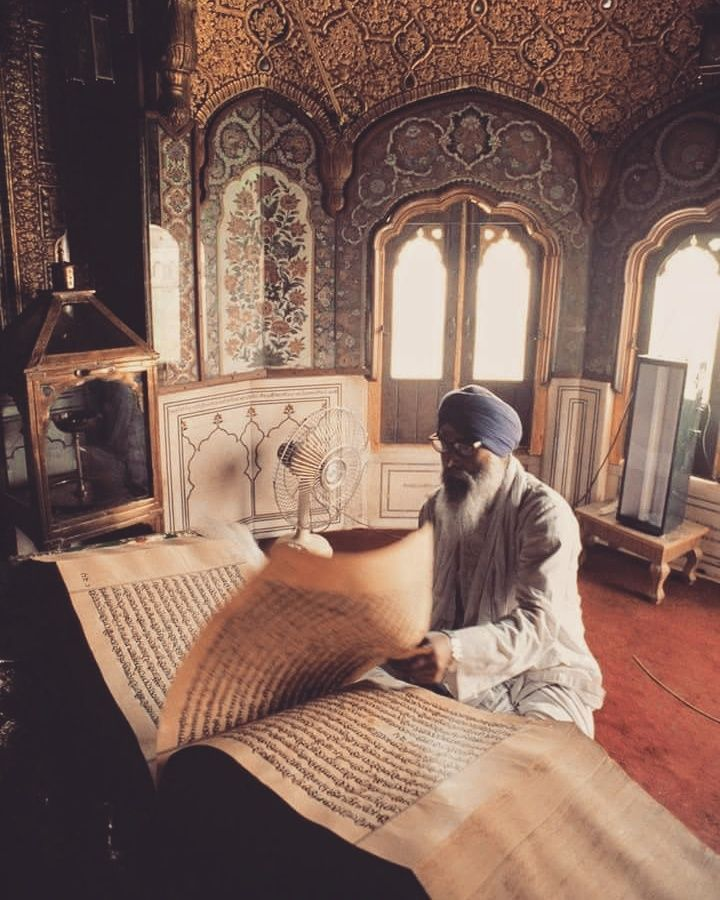
\includegraphics[width=6cm,keepaspectratio]{guru_granth_sahib.jpg}
  \caption{ਸ੍ਰੀ ਗੁਰੂ ਗ੍ਰੰਥ ਸਾਹਿਬ}
\end{figure}
\newpage
\chapter*{ਸ੍ਰੀ ਦਸਮ ਗ੍ਰੰਥ ਸਾਹਿਬ ਜੀ ਦੇ ਸਹਿਜ ਅਤੇ ਅਖੰਡ ਪਾਠ ਦੀ ਮਰਯਾਦਾ}
\addcontentsline{toc}{chapter}{ਸ੍ਰੀ ਦਸਮ ਗ੍ਰੰਥ ਸਾਹਿਬ ਜੀ ਦੇ ਸਹਿਜ ਪਾਠ ਦੀ ਮਰਯਾਦਾ}
\section*{ਆਰੰਭ}
\begin{itemize}
    \item ਅਰਦਾਸ ਕਰਕੇ ਦੇਗ (ਕੜਾਹ ਪ੍ਰਸਾਦ) ਅਤੇ ਸ਼ਰਦਾਈ (ਜਾਂ ਸ਼ਹੀਦੀ ਦੇਗ) ਦਾ ਭੋਗ ਲਵਾ ਕੇ ਹੁਕਮਨਾਮਾ ਸਾਹਿਬ ਲੈਣਾ ਹੈ
    \item ਪਾਠ ਆਰੰਭ ਕਰਨਾ ਹੈ ਅਤੇ ਜਾਪੁ ਸਾਹਿਬ ਦੀ ਸਮਾਪਤੀ ਤੋਂ ਬਾਅਦ ਦੇਗ ਵਰਤਾਉਣੀ ਹੈ
\end{itemize}
\section*{ਮੱਧ}
\begin{itemize}
    \item 33 ਸਵੱਈਏ (ਜਿੱਥੇ "ਤੋ ਤਨ ਤਿਆਗਤ ਹੀ" ਆਉਂਦਾ ਹੈ) ਤੱਕ ਪੜ੍ਹਨਾ ਹੈ
    \item ਜੇਕਰ ਪੋਥੀ ਜਾਂ ਸਰੂਪ ਵਿੱਚ 34 ਸਵੱਈਏ ਹਨ, ਤਾਂ ਪੂਰੇ 34 ("ਜਿਸ ਕੇ ਗੁਰ ਮਸਤਕਿ ਹਾਥੁ ਧਰਿਓ" ਤੱਕ) ਪੜ੍ਹਨੇ ਹਨ
    \item ਇਸ ਤੋਂ ਬਾਅਦ ਅਨੰਦ ਸਾਹਿਬ (ਆਦਿ ਮਹਾਰਾਜ ਵਾਲਾ) ਪੜ੍ਹ ਕੇ ਮੱਧ ਦੀ ਅਰਦਾਸ ਕਰਨੀ ਹੈ
    \item ਦੇਗ ਅਤੇ ਸ਼ਰਦਾਈ ਦਾ ਭੋਗ ਲਵਾਉਣਾ ਹੈ
    \item ਹੁਕਮਨਾਮਾ ਸਾਹਿਬ "ਖਾਲਸਾ ਮਹਿਮਾ" ("ਜੋ ਕਿਛ ਲੇਖ ਲਿਖਿਓ ਬਿਧਨਾ") ਤੋਂ ਲੈਣਾ ਹੈ
\end{itemize}
\newpage
\section*{ਭੋਗ}
\begin{itemize}
    \item 11ਵੀਂ ਅਤੇ 12ਵੀਂ ਹਿਕਾਇਤ ਪੜ੍ਹਨੀ ਹੈ
    \item ਸਮਾਪਤੀ ਤੋਂ ਬਾਅਦ ਇਹ ਬਾਣੀਆਂ ਪੜ੍ਹਨੀਆਂ ਹਨ: ਜਾਪੁ ਸਾਹਿਬ, ਸ਼ਬਦ ਹਜ਼ਾਰੇ (ਪਾ: 10), 33 ਸਵੱਈਏ, ਖਾਲਸਾ ਮਹਿਮਾ ਅਤੇ ਸ਼ਸਤਰ ਨਾਮ ਮਾਲਾ (ਪਹਿਲਾ ਅਧਿਆਇ ਸੰਪੂਰਨ - ਸ੍ਰੀ ਭਗਉਤੀ ਉਸਤਤ)
    \item ਆਰਤੀ ਕਰਨੀ ਹੈ (ਆਦਿ ਮਹਾਰਾਜ ਅਤੇ ਦਸਮ ਮਹਾਰਾਜ ਦੀਆਂ ਬਾਣੀਆਂ ਨਾਲ)
    \item ਅਰਦਾਸ, ਦੇਗ ਤੇ ਸ਼ਰਦਾਈ ਦਾ ਭੋਗ ਅਤੇ ਹੁਕਮਨਾਮਾ ਸਾਹਿਬ ਆਦਿ ਮਹਾਰਾਜ ਵਾਂਗ ਹੀ ਲੈਣਾ ਹੈ
\end{itemize}
\section*{ਅਖੰਡ ਪਾਠ ਵਾਰੇ ਜਰੂਰੀ ਚੀਜ਼ਾਂ }
ਮਰਯਾਦਾ ਦਾ ਵਿਸ਼ੇਸ਼ ਹਿੱਸਾ \textbf{"ਪੰਜ ਤੱਤਾਂ ਦੀ ਮਰਯਾਦਾ"} ਅਤੇ \textbf{"ਸੇਵਾਵਾਂ ਅਤੇ ਸੇਵਾਦਾਰਾਂ ਦਾ ਵੇਰਵਾ"} ਵਾਲੇ ਅੰਗ ਵਿੱਚ ਵਿਸਥਾਰਪੂਰਵਕ ਲਿਖਿਆ ਗਿਆ ਹੈ, ਜਿਸ ਦੀ ਪਾਲਣਾ ਹਰ ਸੇਵਾਦਾਰ ਲਈ ਲਾਜ਼ਮੀ ਹੈ।
\\
\textbf{ਵਿਸ਼ੇਸ਼ ਨੁਕਤਾ: ਸ੍ਰੀ ਜਾਪੁ ਸਾਹਿਬ ਦਾ ਅਖੰਡ ਜਾਪ}
\\
ਇਹ ਵਿਸ਼ੇਸ਼ ਤੌਰ 'ਤੇ ਨੋਟ ਕੀਤਾ ਜਾਵੇ ਕਿ ਮੁੱਖ ਅਖੰਡ ਪਾਠ ਦੇ ਨਾਲ-ਨਾਲ ਸ੍ਰੀ ਜਾਪੁ ਸਾਹਿਬ ਦਾ ਪਾਠ ਵੀ ਨਿਰੰਤਰ ਚੱਲਣਾ ਚਾਹੀਦਾ ਹੈ:
\begin{itemize}
    \item ਜਦੋਂ ਤੱਕ ਅਖੰਡ ਪਾਠ ਸਾਹਿਬ ਜਾਰੀ ਹੈ, ਇੱਕ ਸੇਵਾਦਾਰ ਲਗਾਤਾਰ ਸ੍ਰੀ ਜਪੁਜੀ ਸਾਹਿਬ ਦਾ ਪਾਠ ਕਰੇਗਾ।
    \item ਇੱਕ ਪਾਠ ਸੰਪੂਰਨ ਹੋਣ 'ਤੇ ਅਗਲਾ ਪਾਠ ਤੁਰੰਤ ਸ਼ੁਰੂ ਕੀਤਾ ਜਾਵੇ। ਇਹ ਸਿਲਸਿਲਾ ਭੋਗ ਤੱਕ ਬਿਨਾਂ ਕਿਸੇ ਰੁਕਾਵਟ ਦੇ ਜਾਰੀ ਰਹਿਣਾ ਚਾਹੀਦਾ ਹੈ।
\end{itemize}
\begin{figure}[h]
  \centering
  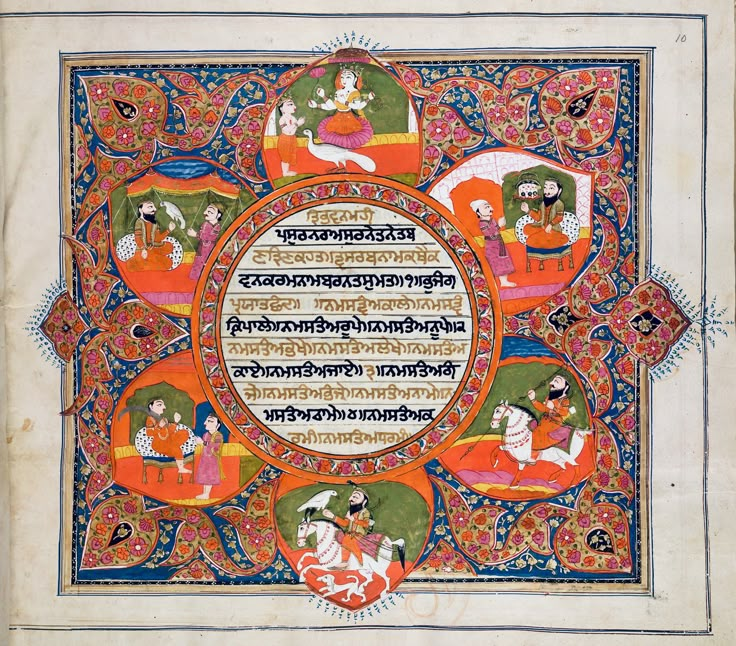
\includegraphics[width=10cm,keepaspectratio]{dasam_granth.jpg}
  \caption{ਸ੍ਰੀ ਦਸਮ ਗ੍ਰੰਥ ਸਾਹਿਬ ਜੀ}
\end{figure}
\newpage
\chapter*{ਸ੍ਰੀ ਸਰਬਲੋਹ ਗ੍ਰੰਥ ਸਾਹਿਬ ਜੀ ਦੇ ਸਹਿਜ ਅਤੇ ਅਖੰਡ ਪਾਠ ਦੀ ਮਰਯਾਦਾ}
\addcontentsline{toc}{chapter}{ਸ੍ਰੀ ਸਰਬਲੋਹ ਗ੍ਰੰਥ ਸਾਹਿਬ ਜੀ ਦੇ ਸਹਿਜ ਪਾਠ ਦੀ ਮਰਯਾਦਾ}
\section*{ਆਰੰਭ}
\begin{itemize}
    \item 405ਵਾਂ ਚਰਿਤਰ (ਸਬੁੱਧ ਬਾਚ) ਸੰਪੂਰਨ ਚੌਪਈ ਸਾਹਿਬ (ਦਸਮ) ਸਮੇਤ ਪੜ੍ਹਨਾ ਹੈ
    \item ਅਰਦਾਸ ਕਰਕੇ ਦੇਗ, ਸ਼ਹੀਦੀ ਦੇਗ/ਸ਼ਰਦਾਈ, 7 ਪ੍ਰਕਾਰ ਦੇ ਭੋਜਨ ਅਤੇ 7 ਪ੍ਰਕਾਰ ਦੇ ਮੇਵਿਆਂ ਦਾ ਭੋਗ ਲਵਾਉਣਾ ਹੈ
    \item 5 ਵਾਰ ਮੂਲ ਮੰਤਰ ਅਤੇ 5 ਵਾਰ "ਅਕਾਲ ਪੁਰਖ ਕੀ ਰੱਛਾ ਹਮਨੈ... ਸਰਬਲੋਹ ਦੀ... ਸਰਬਕਾਲ... ਸਰਬਲੋਹ ਜੀ" (ਦਸਮ ਅਕਾਲ ਉਸਤਤ ਮੰਗਲਾਚਰਨ) ਪੜ੍ਹਨਾ ਹੈ
    \item ਭਵਾਨੀ ਉਸਤਤ ਦੇ 107ਵੇਂ ਛੰਦ 'ਤੇ ਰੁਕਣਾ ਹੈ ਅਤੇ ਦੇਗ ਵਰਤਾਉਣੀ ਹੈ
\end{itemize}
\section*{ਮੱਧ}
\begin{itemize}
    \item 2861ਵੇਂ ਛੰਦ ਤੱਕ ਪੜ੍ਹ ਕੇ ਰੁਕਣਾ ਹੈ
    \item ਸਰਬਲੋਹ ਮਹਾਰਾਜ ਦਾ ਅਨੰਦ ਸਾਹਿਬ ("ਥਾਰ੍ਹੋ ਅਚਰਨ ਹਿਤ ਜਗ ਤਰਨ..." ਛੰਦ 3063-3077) ਪੜ੍ਹਨਾ ਹੈ
    \item ਆਰਤੀ (ਸਰਬਲੋਹ ਜੀ ਦੀ ਵੱਖਰੀ ਆਰਤੀ ਜੋ ਦਿਵਾਲੀ ਮਹਾਤਮ ਪੋਥੀ ਵਿੱਚ ਹੈ) ਅਤੇ ਆਦਿ ਮਹਾਰਾਜ ਵਾਲਾ ਅਨੰਦ ਸਾਹਿਬ ਪੜ੍ਹਨਾ ਹੈ
    \item ਅਰਦਾਸ, ਦੇਗ ਅਤੇ 7 ਪ੍ਰਕਾਰ ਦੇ ਭੋਜਨ/ਮੇਵਿਆਂ ਦਾ ਭੋਗ ਲਵਾਉਣਾ ਹੈ
    \item ਹੁਕਮਨਾਮਾ ਸਾਹਿਬ ਸਰਬਲੋਹ ਅਸਤੋਤਰ (ਛੰਦ 2862, 2863) ਤੋਂ ਲੈਣਾ ਹੈ
\end{itemize}
\newpage
\section*{ਭੋਗ}
\begin{itemize}
    \item 1425ਵਾਂ ਛੰਦ "ਅਪਕਰਮਨ ਕੋ ਫਲ" ਤੋਂ ਅਖੀਰ ਤੱਕ ਸੁਰ ਵਿੱਚ ਪੜ੍ਹਨਾ ਹੈ
    \item ਸ਼੍ਰੀ ਭਵਾਨੀ 1-107 ਛੰਦ, ਗੁਰਗੱਦੀ ਪਾਤਸ਼ਾਹੀ ਦਸਵੀਂ (ਛੰਦ 3159 ਤੋਂ 3162, 3163, 3164 ਖਾਲਸਾ ਪ੍ਰਕਾਸ਼ ਸਵੱਈਏ) ਪੜ੍ਹਨੇ ਹਨ
    \item ਖਾਲਸਾ ਮਹਿਮਾ (3308-3310), ਸਰਬਲੋਹ ਕਵਚ (2877) ਅਤੇ ਸਰਬਲੋਹ ਅਸਤੋਤਰ (2862-63) ਪੜ੍ਹਨਾ ਹੈ
    \item ਦੁਬਾਰਾ ਸਰਬਲੋਹ ਅਨੰਦ ਸਾਹਿਬ (3063-3077) ਪੜ੍ਹਨਾ ਹੈ
    \item ਆਰਤੀ ਕਰਨੀ ਹੈ (ਆਦਿ ਮਹਾਰਾਜ, ਦਸਮ ਮਹਾਰਾਜ ਅਤੇ ਸਰਬਲੋਹ ਮਹਾਰਾਜ ਦੀਆਂ ਬਾਣੀਆਂ ਨਾਲ)
    \item ਇਹ ਦਲ ਪੰਥਾਂ ਦੁਆਰਾ ਪ੍ਰਮਾਣਿਤ ਵਿਧੀ ਹੈ । ਇੱਕ ਹੋਰ ਤਰੀਕਾ ਹਰ ਅਧਿਆਏ (ਕੁੱਲ 5 ਅਧਿਆਏ) ਦੀ ਸਮਾਪਤੀ 'ਤੇ ਜਸ਼ਨ ਮਨਾਉਣ ਅਤੇ ਭੋਗ ਪਾਉਣ ਦਾ ਵੀ ਹੈ
\end{itemize}
\section*{ਅਖੰਡ ਪਾਠ ਵਾਰੇ ਜਰੂਰੀ ਚੀਜ਼ਾਂ }
ਮਰਯਾਦਾ ਦਾ ਵਿਸ਼ੇਸ਼ ਹਿੱਸਾ \textbf{"ਪੰਜ ਤੱਤਾਂ ਦੀ ਮਰਯਾਦਾ"} ਅਤੇ \textbf{"ਸੇਵਾਵਾਂ ਅਤੇ ਸੇਵਾਦਾਰਾਂ ਦਾ ਵੇਰਵਾ"} ਵਾਲੇ ਅੰਗ ਵਿੱਚ ਵਿਸਥਾਰਪੂਰਵਕ ਲਿਖਿਆ ਗਿਆ ਹੈ, ਜਿਸ ਦੀ ਪਾਲਣਾ ਹਰ ਸੇਵਾਦਾਰ ਲਈ ਲਾਜ਼ਮੀ ਹੈ।
\\
\textbf{ਵਿਸ਼ੇਸ਼ ਨੁਕਤਾ: ਉਸਤਤ ਮਾਯਾ ਲਕਸ਼ਮੀ ਦਾ ਅਖੰਡ ਜਾਪ}
\\
ਇਹ ਵਿਸ਼ੇਸ਼ ਤੌਰ 'ਤੇ ਨੋਟ ਕੀਤਾ ਜਾਵੇ ਕਿ ਮੁੱਖ ਅਖੰਡ ਪਾਠ ਦੇ ਨਾਲ-ਨਾਲ ਉਸਤਤ ਮਾਯਾ ਲਕਸ਼ਮੀ ਦਾ ਪਾਠ ਵੀ ਨਿਰੰਤਰ ਚੱਲਣਾ ਚਾਹੀਦਾ ਹੈ:
\begin{itemize}
    \item ਜਦੋਂ ਤੱਕ ਅਖੰਡ ਪਾਠ ਸਾਹਿਬ ਜਾਰੀ ਹੈ, ਇੱਕ ਸੇਵਾਦਾਰ ਲਗਾਤਾਰ ਸ੍ਰੀ ਜਪੁਜੀ ਸਾਹਿਬ ਦਾ ਪਾਠ ਕਰੇਗਾ।
    \item ਇੱਕ ਪਾਠ ਸੰਪੂਰਨ ਹੋਣ 'ਤੇ ਅਗਲਾ ਪਾਠ ਤੁਰੰਤ ਸ਼ੁਰੂ ਕੀਤਾ ਜਾਵੇ। ਇਹ ਸਿਲਸਿਲਾ ਭੋਗ ਤੱਕ ਬਿਨਾਂ ਕਿਸੇ ਰੁਕਾਵਟ ਦੇ ਜਾਰੀ ਰਹਿਣਾ ਚਾਹੀਦਾ ਹੈ।
\end{itemize}
\begin{figure}[h]
  \centering
  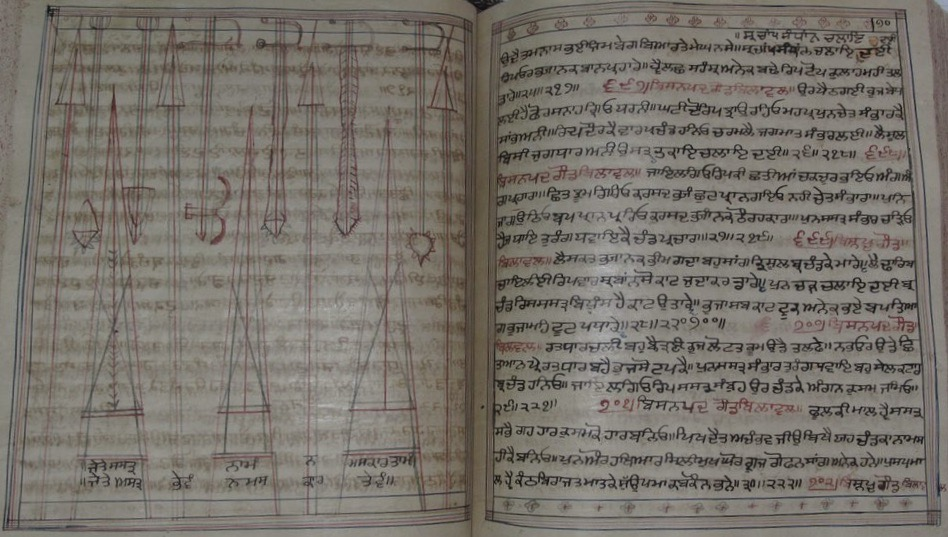
\includegraphics[width=10cm,keepaspectratio]{sarblo_granth.jpg}
  \caption{ਸ੍ਰੀ ਸਰਬਲੋਹ ਗ੍ਰੰਥ ਸਾਹਿਬ ਜੀ}
\end{figure}
\newpage
\chapter*{ਹੁਕਮਨਾਮਾ ਲੈਣ ਦੀ ਮਰਯਾਦਾ}
\addcontentsline{toc}{chapter}{ਹੁਕਮਨਾਮਾ ਲੈਣ ਦੀ ਮਰਯਾਦਾ}
\begin{itemize}
    \item \textbf{ਅੰਮ੍ਰਿਤ ਵੇਲਾ (ਪ੍ਰਕਾਸ਼ ਵੇਲੇ):} ਖੱਬੇ ਪਾਸੇ ਤੋਂ ਉਹ ਸ਼ਬਦ ਜੋ ਚੱਲ ਰਿਹਾ ਹੈ। ਜੇਕਰ ਉਹ ਸ਼ਬਦ ਉੱਪਰੋਂ ਸ਼ੁਰੂ ਹੋ ਰਿਹਾ ਹੈ (ਜਿਵੇਂ: ਆਸਾ ਮਹਲਾ, ਗੁਜਰੀ ਮਹਲਾ), ਤਾਂ ਉੱਥੋਂ ਲਓ। ਜੇਕਰ ਸ਼ਬਦ ਪਿਛਲੇ ਅੰਗ ਤੋਂ ਸ਼ੁਰੂ ਹੋਇਆ ਹੈ, ਤਾਂ ਅੰਗ ਪਰਤ ਕੇ ਸ਼ਬਦ ਦੇ ਆਰੰਭ ਤੋਂ ਪੜ੍ਹਨਾ ਸ਼ੁਰੂ ਕਰੋ
    \item \textbf{ਦੁਪਹਿਰ ਵੇਲੇ:} ਖੱਬੇ ਪਾਸੇ ਦੇ ਅੰਗ ਦੇ ਅਖੀਰ ਤੋਂ ਸ਼ੁਰੂ ਹੋ ਕੇ ਸੱਜੇ ਪਾਸੇ ਦੇ ਅੰਗ ਦੇ ਉੱਪਰ ਖਤਮ ਹੋਣ ਵਾਲਾ ਸ਼ਬਦ
    \item \textbf{ਸ਼ਾਮ ਵੇਲੇ:} ਸੱਜੇ ਪਾਸੇ ਦੇ ਅੰਗ ਦਾ ਉਹ ਸ਼ਬਦ ਜੋ ਉਸੇ ਅੰਗ 'ਤੇ ਖਤਮ ਹੁੰਦਾ ਹੋਵੇ (ਦੂਜਾ ਆਖਰੀ ਸ਼ਬਦ ਜਾਂ ਕਈ ਵਾਰ ਆਖਰੀ ਸ਼ਬਦ ਜੇ ਉਹ ਉਸੇ ਅੰਗ 'ਤੇ ਸੰਪੂਰਨ ਹੁੰਦਾ ਹੈ)
\end{itemize}
\begin{figure}[h]
  \centering
  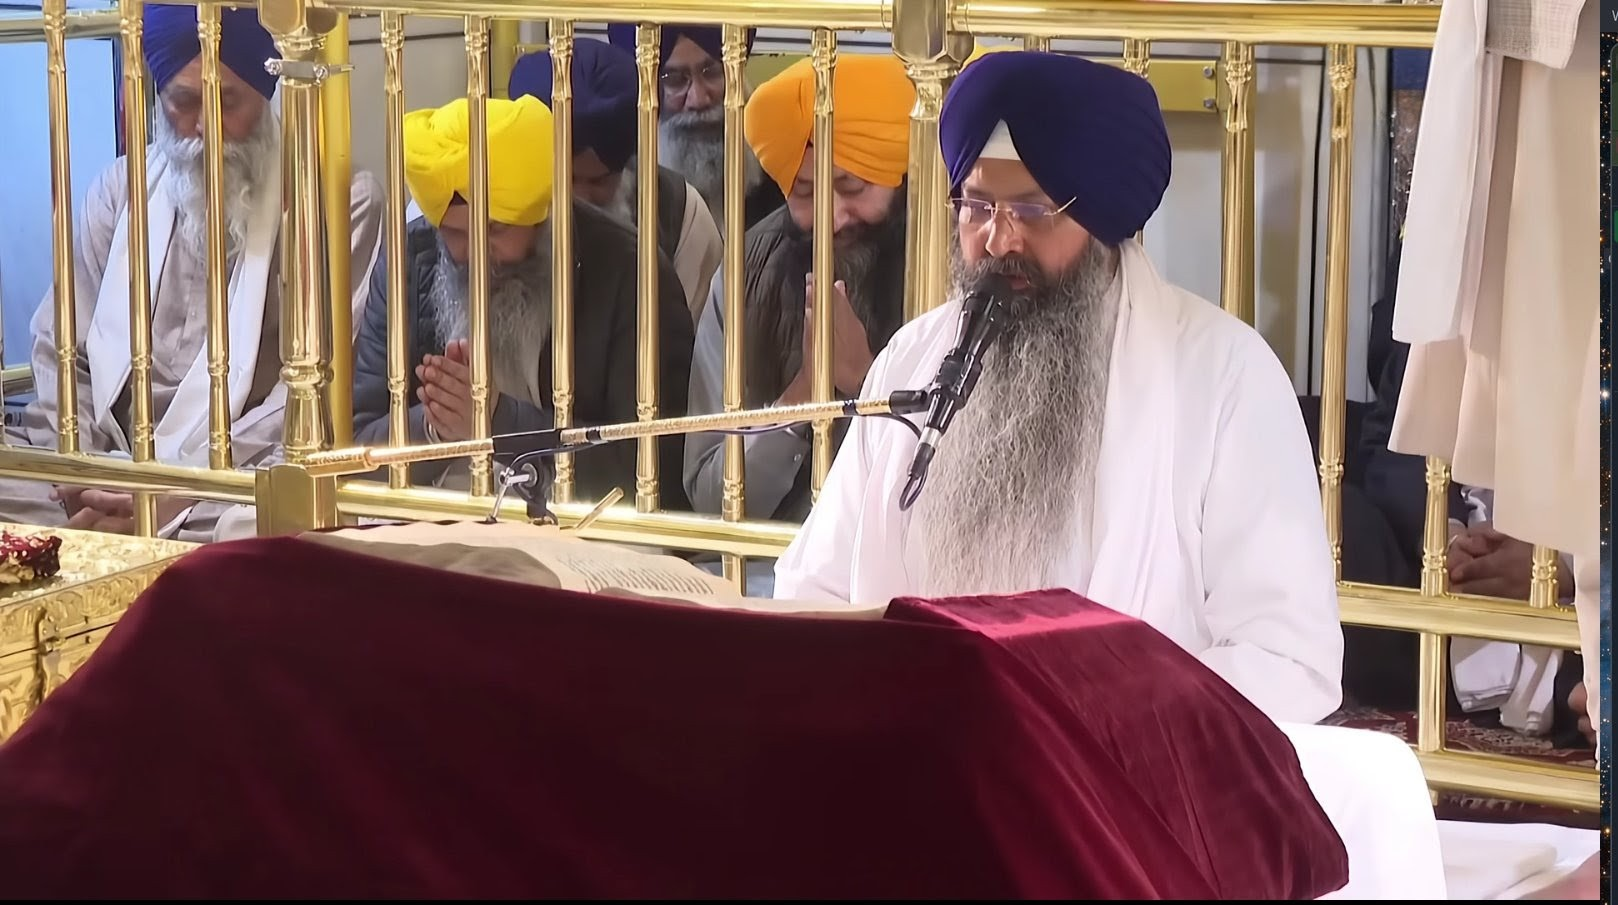
\includegraphics[width=10cm,keepaspectratio]{hukumnama.png}
  \caption{ਹੁਕਮਨਾਮਾ ਲੈਣ ਦੀ ਮਰਯਾਦਾ)}
\end{figure}
\newpage
\thispagestyle{empty} % Optional: Removes page number from this specific page
\vspace*{\fill}

\begin{center}
    {\Huge \textbf{ਚਿੱਤਰ ਸੰਗ੍ਰਹਿ}} % The title
    \addcontentsline{toc}{chapter}{ਚਿੱਤਰ ਸੰਗ੍ਰਹਿ} % Adds it to the TOC
\end{center}

\vspace*{\fill}
\begin{figure}[p]
  \thispagestyle{empty}  % No page number
  \centering
  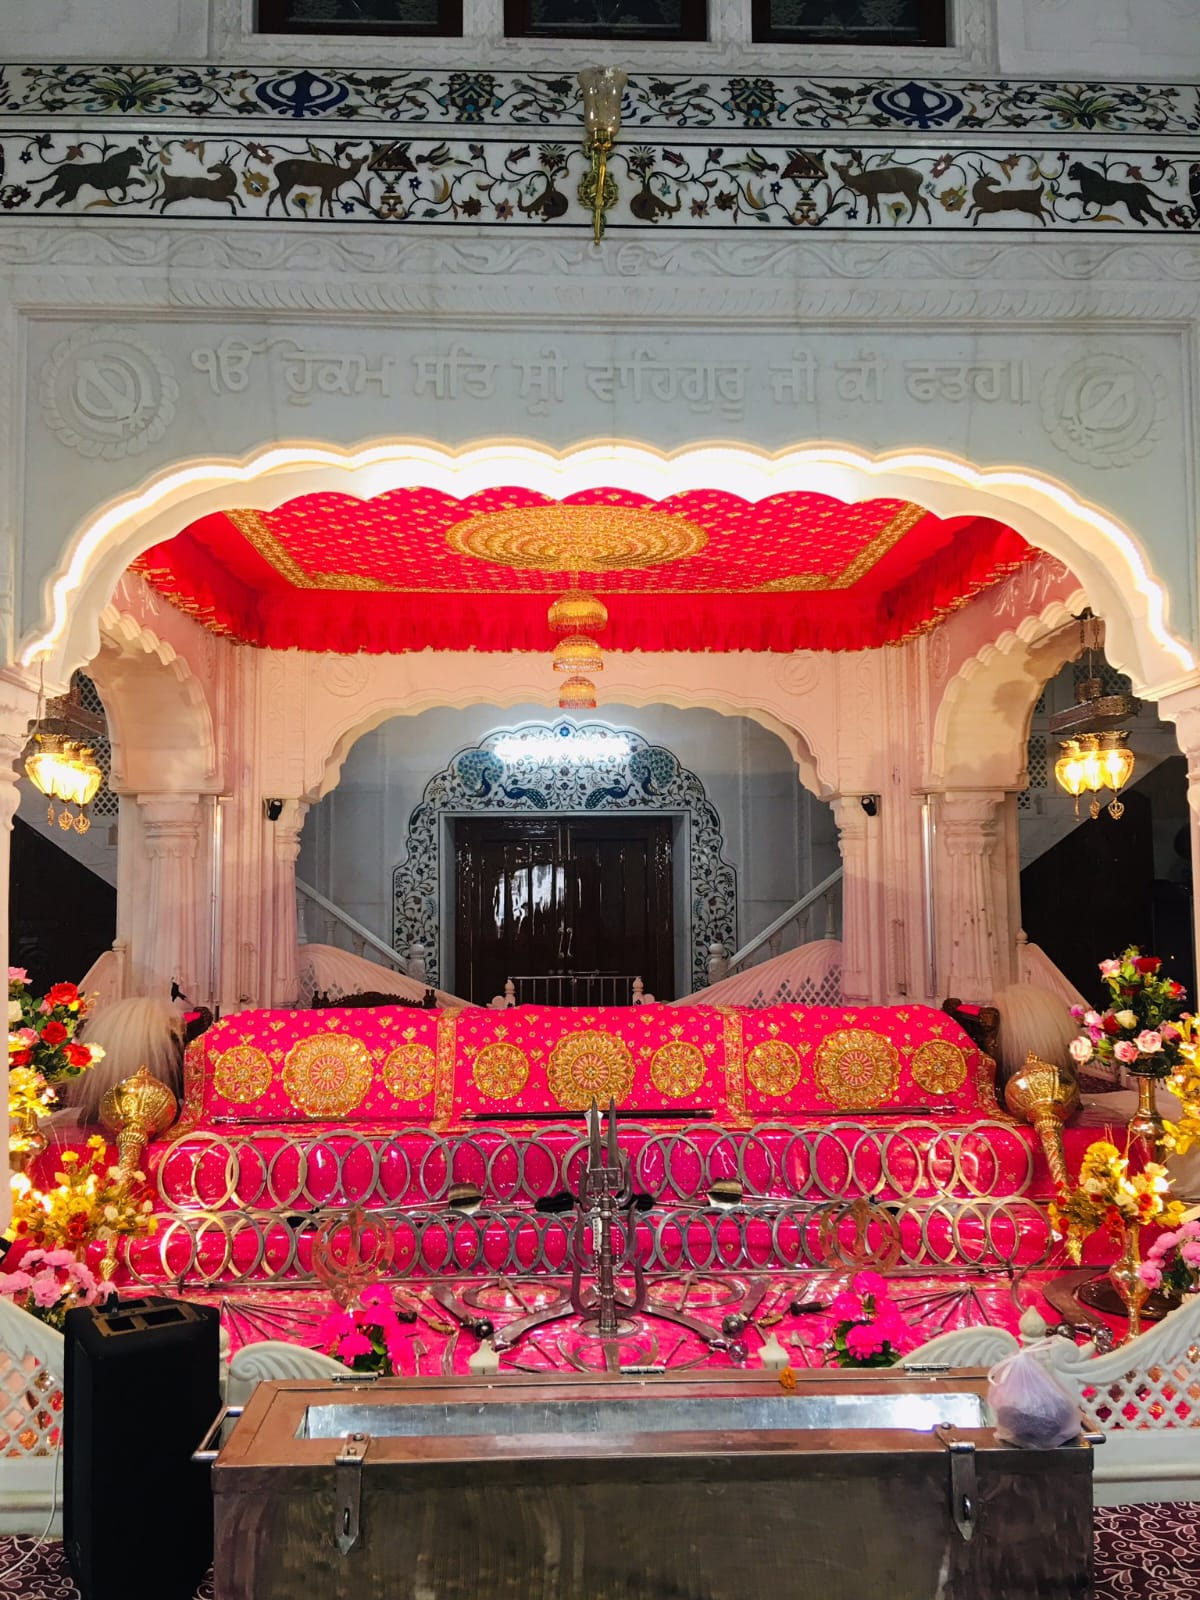
\includegraphics[width=\textwidth,height=0.85\textheight,keepaspectratio]{katha_prakash.jpeg}
  \vspace{1em}
  \caption{ਸ੍ਰੀ ਗੁਰੂ ਗ੍ਰੰਥ ਸਾਹਿਬ, ਸ੍ਰੀ ਦਸਮ ਗ੍ਰੰਥ ਸਾਹਿਬ ਅਤੇ ਸ੍ਰੀ ਸਰਬਲੋਹ ਗ੍ਰੰਥ ਸਾਹਿਬ ਜੀ ਦਾ ਕਥਾ ਪ੍ਰਕਾਸ਼ (ਸ਼ਹੀਦੀ ਬਾਗ਼, ਸ੍ਰੀ ਅਨੰਦਪੁਰ ਸਾਹਿਬ ਵਿਖੇ)}
\end{figure}
\clearpage
\begin{figure}[p]
  \thispagestyle{empty}  % No page number
  \centering
  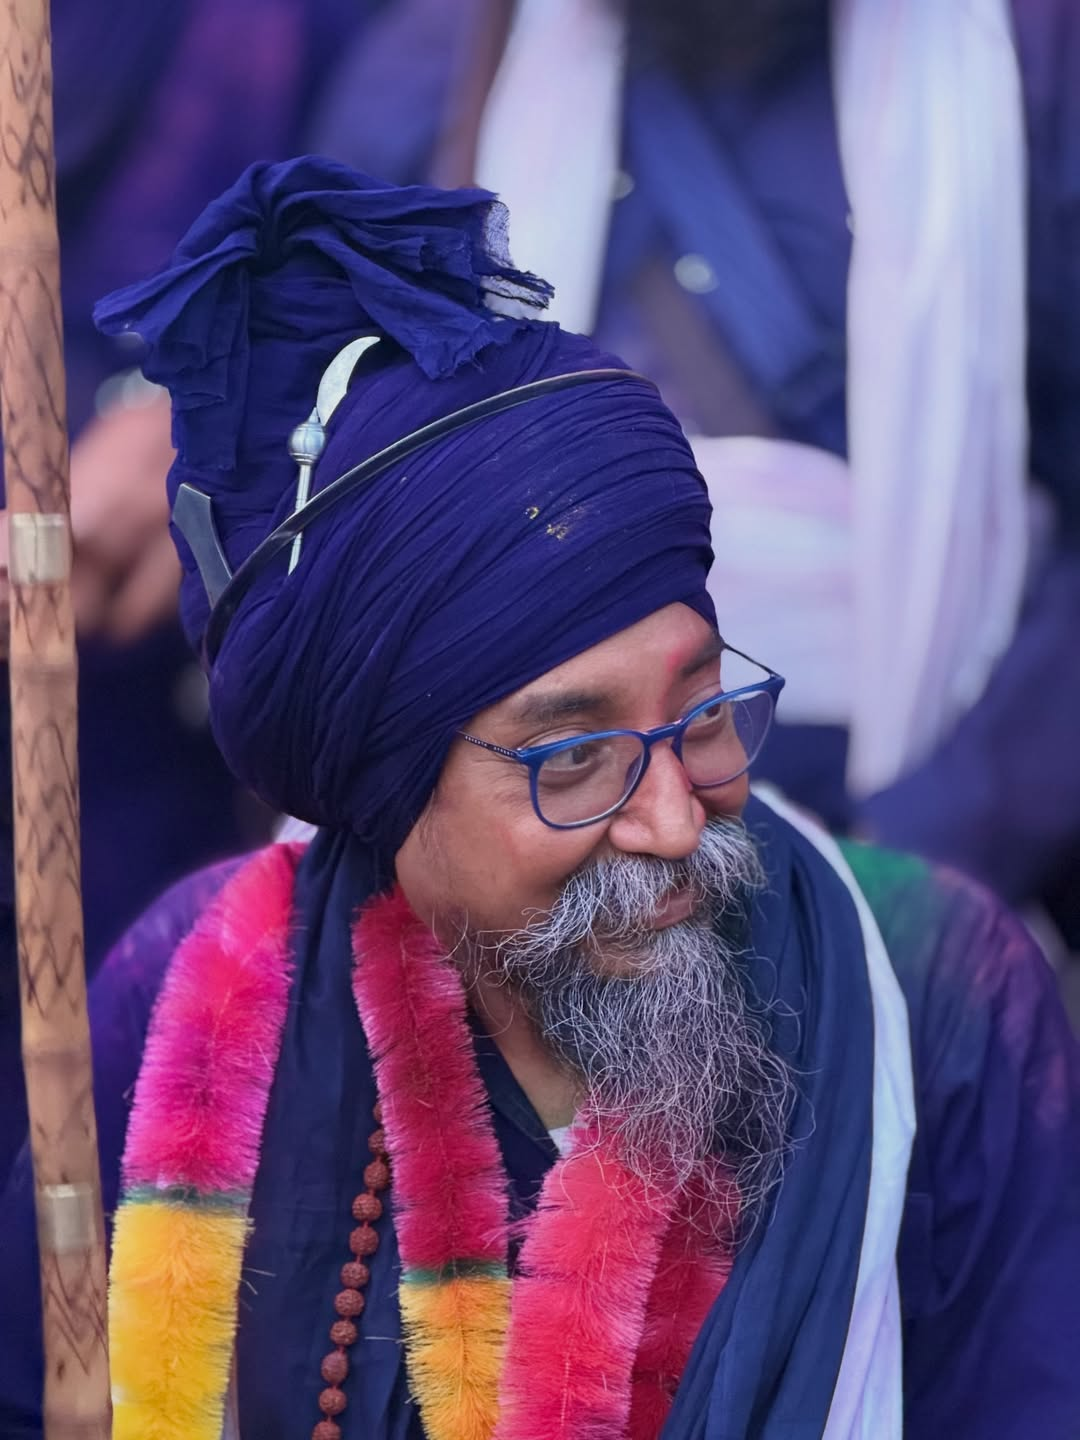
\includegraphics[width=\textwidth,height=0.85\textheight,keepaspectratio]{giani_sher_singh.jpg}
  \vspace{1em}
  \caption{ਮਹਾਕਾਲ ਬਾਬਾ ਗਿਆਨੀ ਸ਼ੇਰ ਸਿੰਘ ਜੀ}
\end{figure}
\clearpage
\begin{figure}[p]
  \thispagestyle{empty}  % No page number
  \centering
  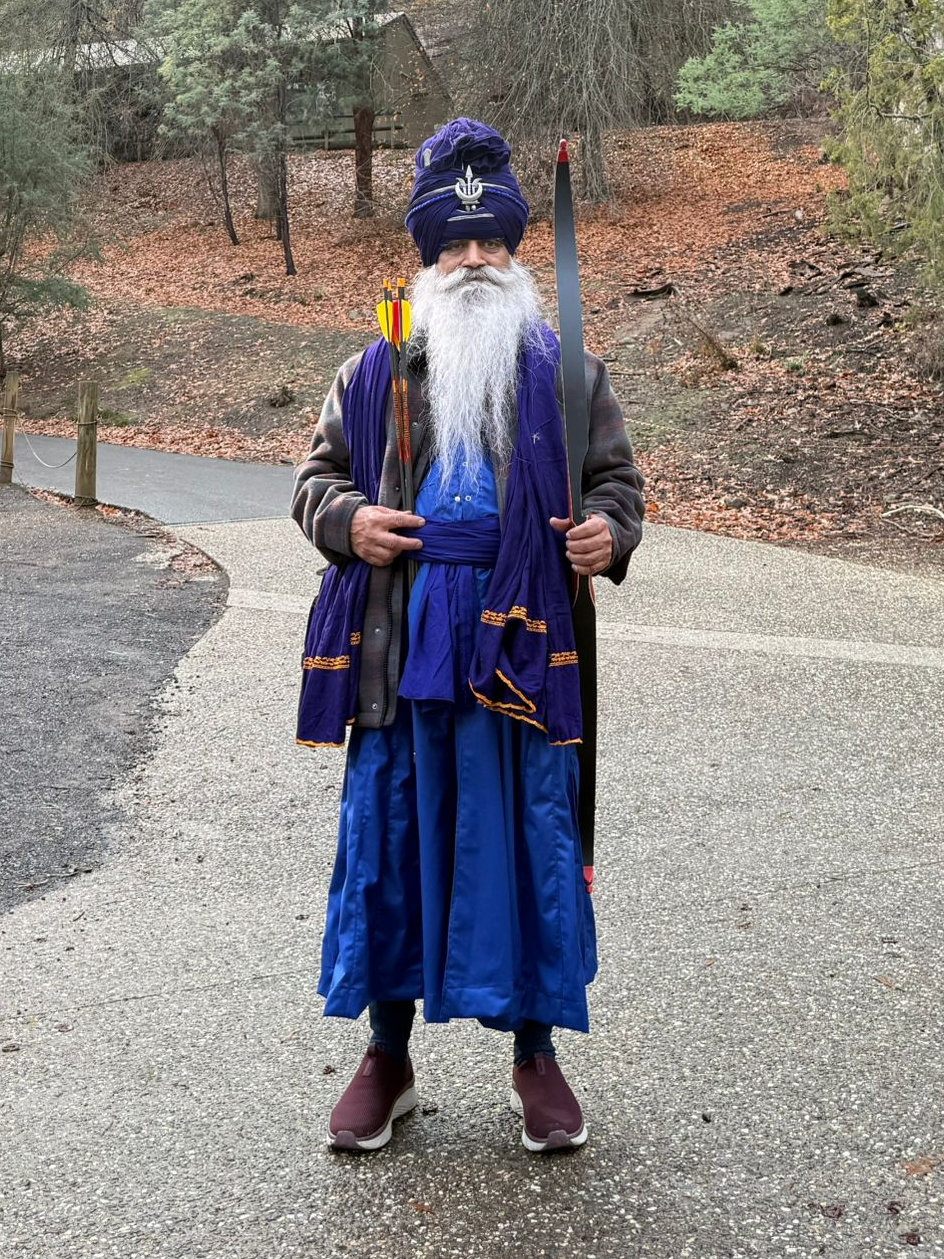
\includegraphics[width=\textwidth,height=0.85\textheight,keepaspectratio]{giani_sukha_singh_ji.jpeg}
  \vspace{1em}
  \caption{ਮਹਾਕਾਲ ਬਾਬਾ ਸੁੱਖਾ ਸਿੰਘ ਜੀ}
\end{figure}
\clearpage
\begin{figure}[p]
  \thispagestyle{empty}  % No page number
  \centering
  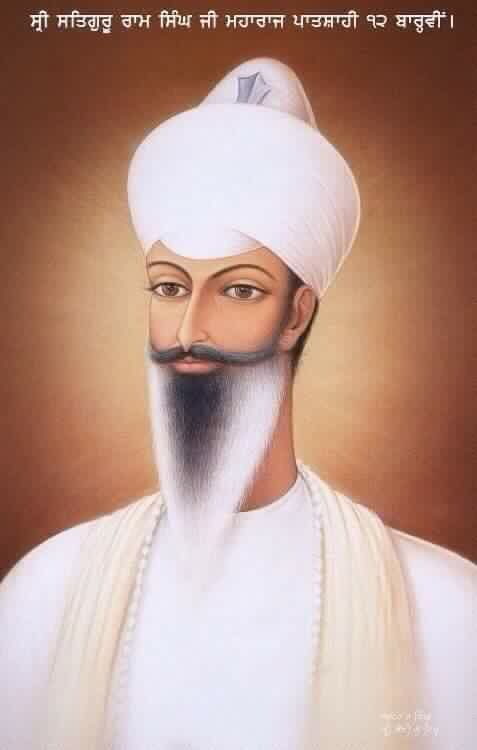
\includegraphics[width=\textwidth,height=0.85\textheight,keepaspectratio]{satguru_ram_singh_ji.jpg}
  \vspace{1em}
  \caption{ ਸ਼੍ਰੀ ਸਤਿਗੁਰੂ ਰਾਮ ਸਿੰਘ ਜੀ}
\end{figure}
\clearpage
\begin{figure}[p]
  \thispagestyle{empty}  % No page number
  \centering
  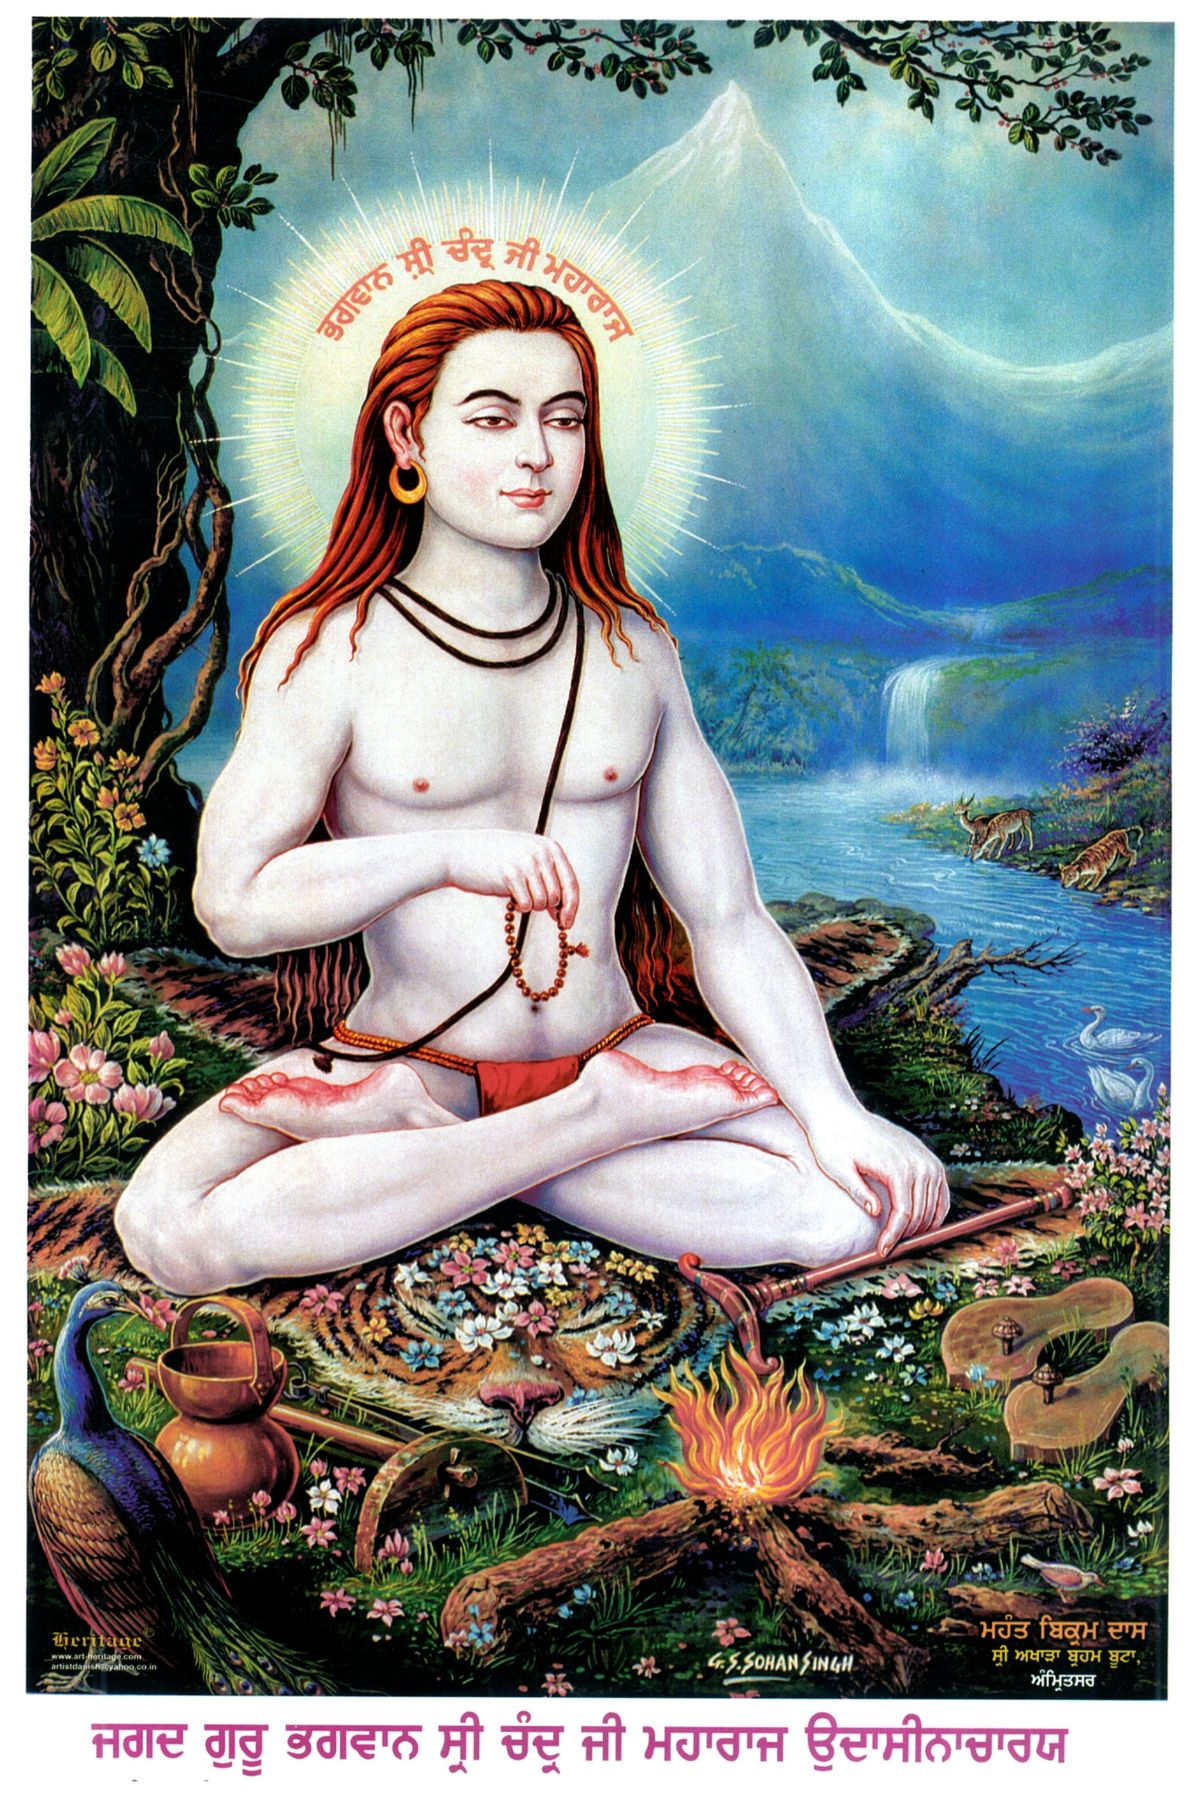
\includegraphics[width=\textwidth,height=0.85\textheight,keepaspectratio]{baba_shri_chand_ji.jpg}
  \vspace{1em}
  \caption{ ਬਾਬਾ ਸ਼੍ਰੀ ਚੰਦ ਜੀ}
\end{figure}
\clearpage
\begin{figure}[p]
  \thispagestyle{empty}  % No page number
  \centering
  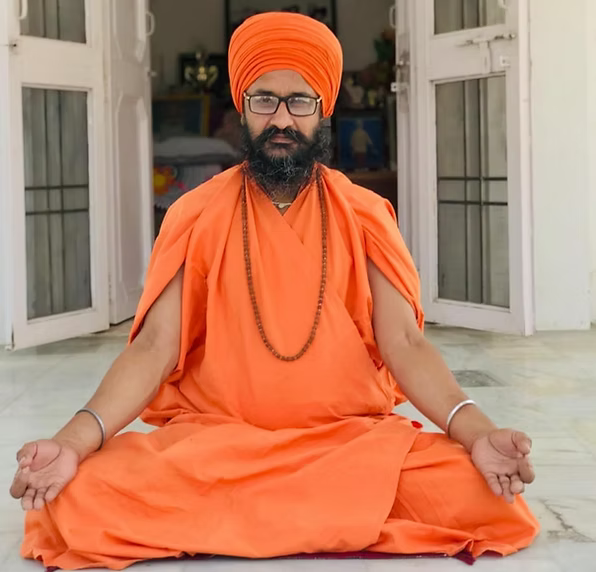
\includegraphics[width=\textwidth,height=0.85\textheight,keepaspectratio]{sant_darshan_singh_ji_sashtri.png}
  \vspace{1em}
  \caption{ ਸੰਤ ਦਰਸ਼ਨ ਸਿੰਘ ਜੀ ਸ਼ਾਸਤਰੀ }
\end{figure}
\clearpage
\begin{figure}[p]
  \thispagestyle{empty}  % No page number
  \centering
  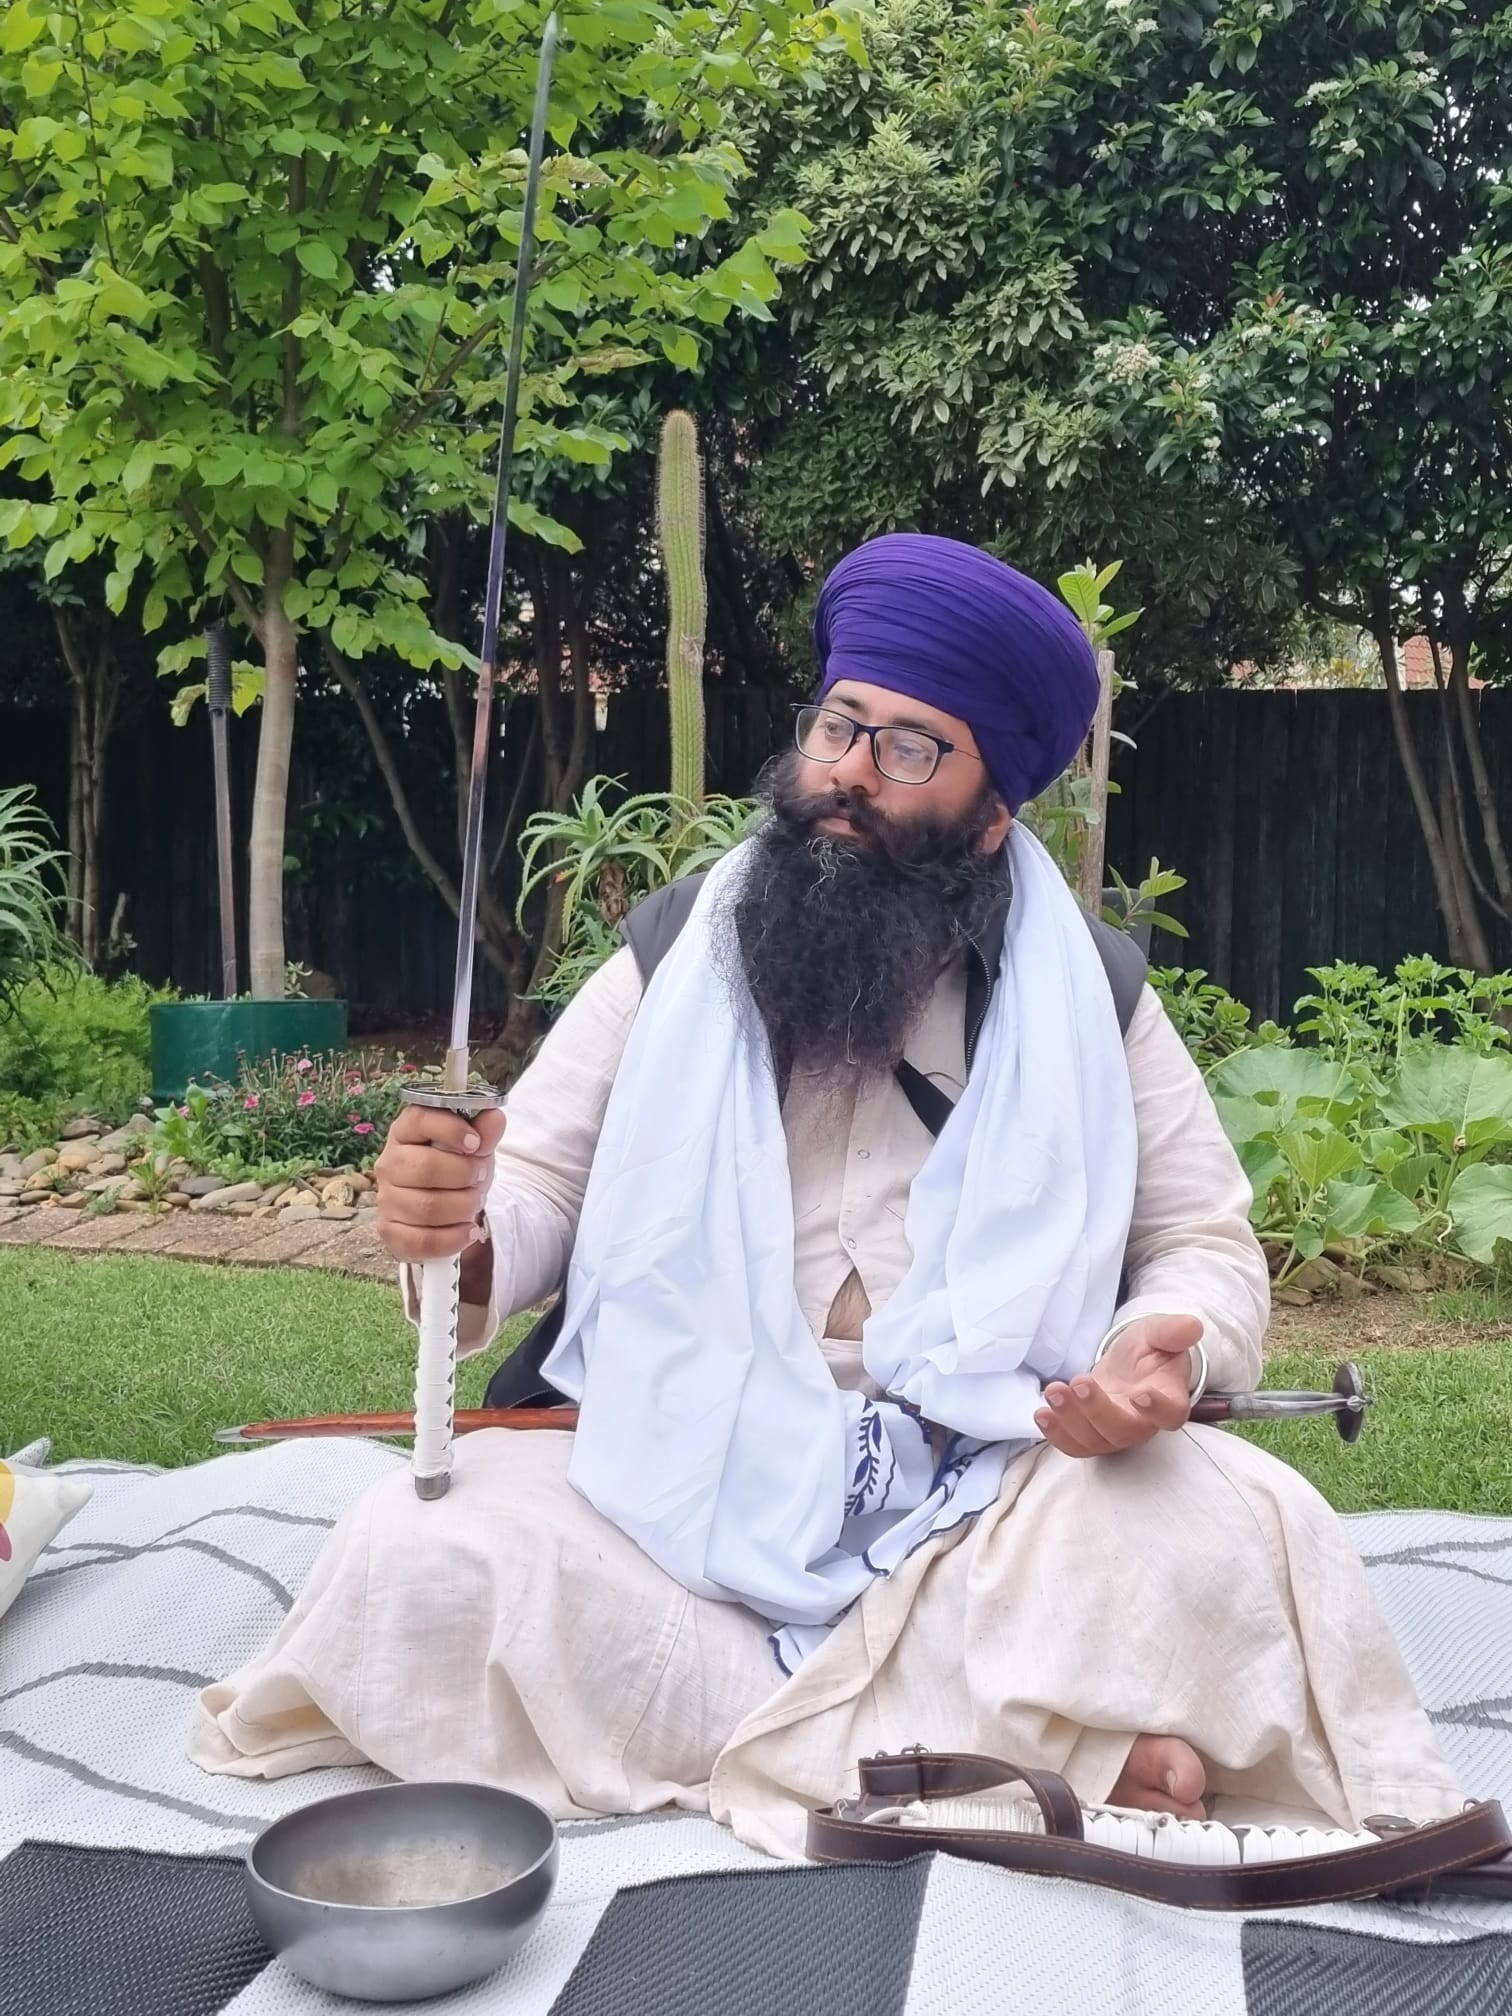
\includegraphics[width=\textwidth,height=0.85\textheight,keepaspectratio]{giani_gurvinder_singh_nangli.jpeg}
  \vspace{1em}
  \caption{ਗਿਆਨੀ ਗੁਰਵਿੰਦਰ ਸਿੰਘ ਜੀ ਮੁਖ ਸੇਵਾਦਾਰ ਸ੍ਰੀ ਸਰਬਲੋਹ ਬੁੰਗਾ ਨੰਗਲੀ ਸਾਹਿਬ}
\end{figure}
\clearpage
\begin{figure}[p]
  \thispagestyle{empty}  % No page number
  \centering
  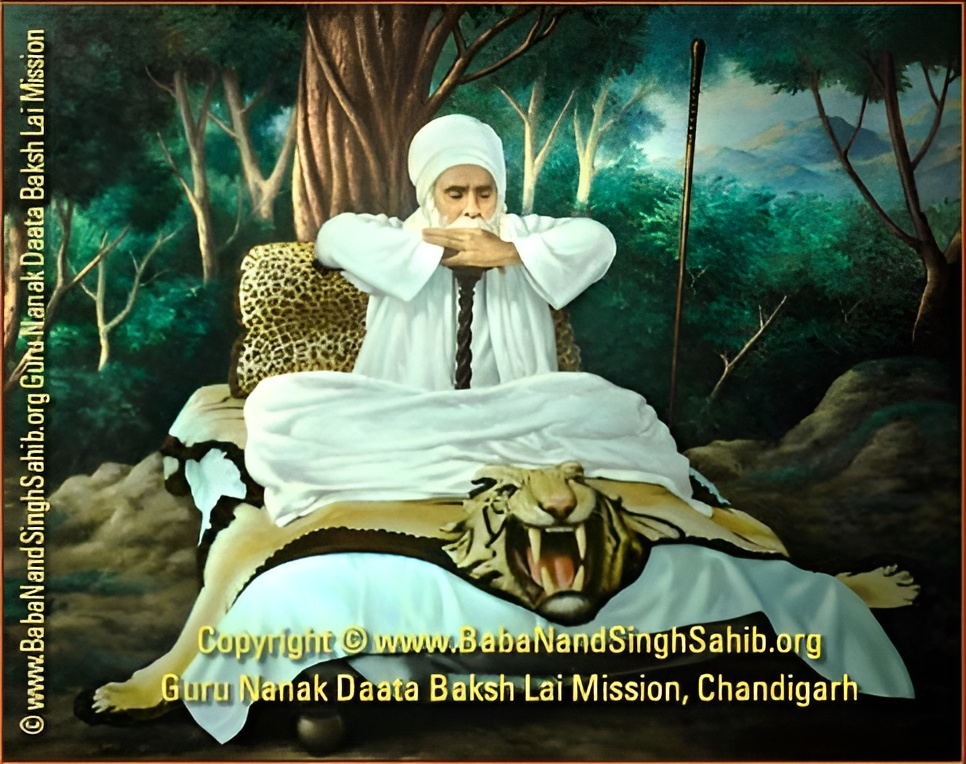
\includegraphics[width=\textwidth,height=0.85\textheight,keepaspectratio]{baba_nand_singh_ji.jpeg}
  \vspace{1em}
  \caption{ ਬਾਬਾ ਨੰਦ ਸਿੰਘ ਜੀ  }
\end{figure}
\clearpage
\begin{figure}[p]
  \thispagestyle{empty}  % No page number
  \centering
  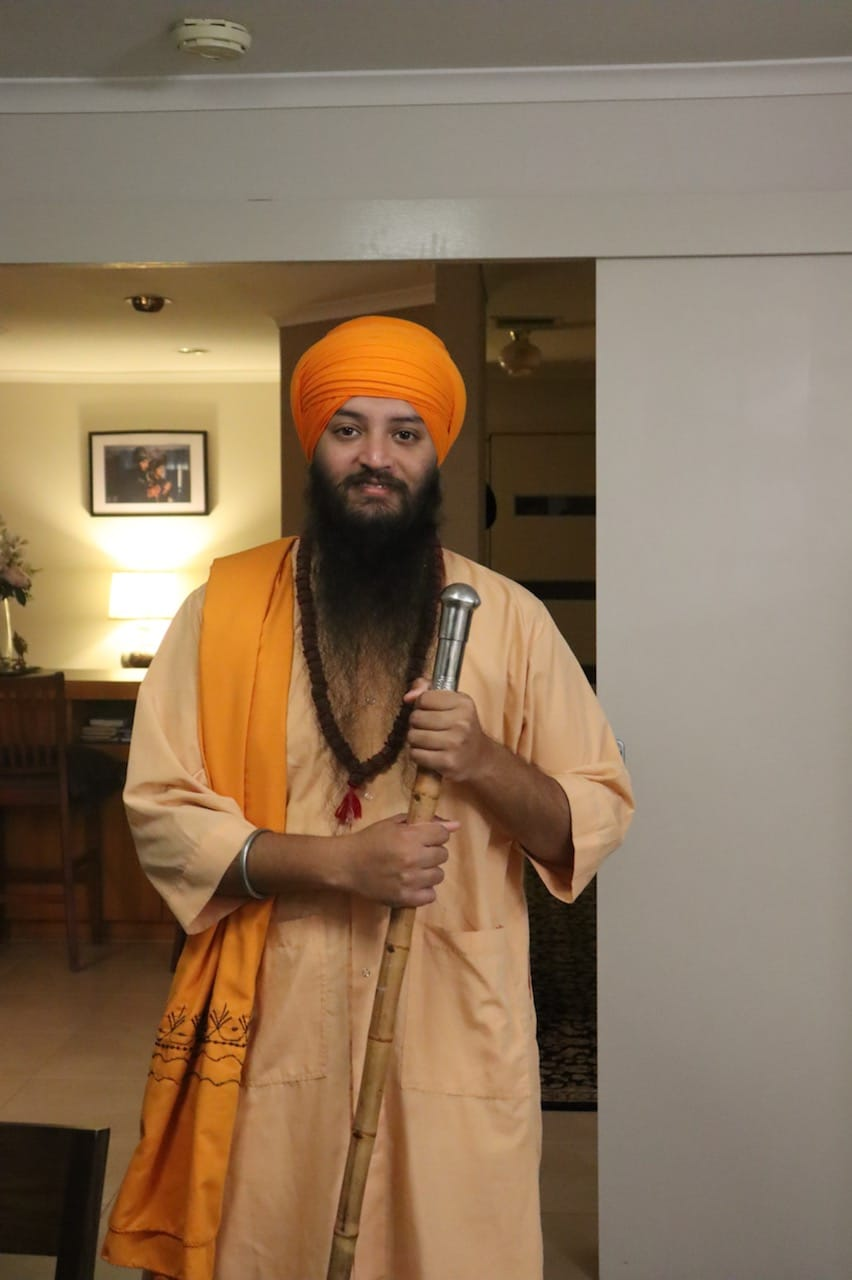
\includegraphics[width=\textwidth,height=0.85\textheight,keepaspectratio]{bhai_manpreet_singh_ji.jpeg}
  \vspace{1em}
  \caption{ਭਾਈ ਮਨਪ੍ਰੀਤ ਸਿੰਘ}
\end{figure}
\end{document}
